\documentclass[11pt,a4paper]{article}

\usepackage[utf8]{inputenc}
\usepackage[T1]{fontenc}
\usepackage{lmodern}
\usepackage{textcomp}
\usepackage{amsmath,amssymb}
\usepackage{algorithm}
\usepackage{algpseudocode}
\usepackage{booktabs}
\usepackage[authoryear,round]{natbib}
\usepackage{hyperref}
\usepackage{listings}
\usepackage{needspace}
\usepackage{etoolbox}
% A short listing must not split across a page: ask for room before it starts.
\BeforeBeginEnvironment{lstlisting}{\needspace{6\baselineskip}}
\usepackage{xcolor}
\usepackage[margin=2.5cm]{geometry}
\usepackage{enumitem}
\usepackage{graphicx}
\usepackage{tikz}
\usetikzlibrary{arrows.meta,positioning,shapes.geometric,calc,fit,backgrounds}
\setlength{\parskip}{0.4em}
\setlength{\parindent}{0em}

\hypersetup{
    colorlinks=true,
    linkcolor=blue!60!black,
    citecolor=blue!60!black,
    urlcolor=blue!60!black
}

\definecolor{codebg}{HTML}{F5F5F5}
\definecolor{teal}{HTML}{0D9488}
\definecolor{violet}{HTML}{A78BFA}
\definecolor{amber}{HTML}{FBBF24}

\tikzset{
    diag title/.style={font=\sffamily\small\bfseries},
    diag box/.style={
        draw=black!75,
        rounded corners=1.5pt,
        fill=gray!4,
        minimum height=0.82cm,
        minimum width=2.5cm,
        align=center,
        font=\sffamily\small,
        inner sep=4pt
    },
    diag data/.style={diag box, rounded corners=0.5pt, fill=gray!8},
    diag ai/.style={diag box, rounded corners=4pt, fill=gray!11},
    diag det/.style={diag box, rounded corners=0.5pt, fill=gray!12, line width=1.0pt},
    diag out/.style={diag box, fill=white},
    diag header/.style={diag box, fill=gray!10, font=\ttfamily\small},
    diag decision/.style={
        draw=black!75,
        diamond,
        aspect=2.35,
        fill=white,
        inner sep=2pt,
        align=center,
        font=\sffamily\scriptsize
    },
    diag terminal/.style={
        draw=black!75,
        rounded corners=1.5pt,
        fill=gray!2,
        minimum height=0.7cm,
        minimum width=1.95cm,
        align=center,
        font=\sffamily\scriptsize\bfseries,
        inner sep=4pt
    },
    diag code/.style={font=\ttfamily\scriptsize, align=left},
    diag note/.style={font=\sffamily\scriptsize, text=black!70, align=center},
    diag label/.style={font=\sffamily\scriptsize, text=black!60},
    diag arrow/.style={-{Stealth[length=4pt]}, semithick, draw=black!70},
    diag feedback/.style={-{Stealth[length=4pt]}, dashed, semithick, draw=black!60}
}

\lstset{
    upquote=true,
    basicstyle=\small\ttfamily,
    backgroundcolor=\color{codebg},
    frame=single,
    framerule=0.5pt,
    rulecolor=\color{gray!30},
    breaklines=true,
    columns=flexible,
    keepspaces=true,
    tabsize=2
}


\title{\textbf{ProveML: Inline Claim Markup for Deterministic Verification of AI-Generated Text}\\[0.3em]\large Technical Report}
\author{Shane Deconinck\\\small{abovebeyond.ai}\\\small{\texttt{hello@shanedeconinck.be}}}
\date{August 2026}

\begin{document}

\maketitle

\begin{center}
\fbox{\parbox{0.92\textwidth}{\small\textbf{Note (August 2026).} This report holds the complete specification and the July 2026 study of four small local models, with a substitution baseline and two ablations. The short paper of August 2026 reports a study of three frontier models and supersedes the evaluation here as the paper's evidence. Two things changed in the specification after this report was written: a fact may name its own record (\texttt{\%[student:20414.passRate]\{53\}}), and the verifier reports coverage. One thing changed in how this study should be read: the context handed to the models named two fields (\texttt{students}, \texttt{rate}) differently from the store (\texttt{studentCount}, \texttt{passRate}), which inflated the addressability errors reported below; the short paper documents the mismatch and the corrected harness.}}
\end{center}


\begin{abstract}
Organizations are deploying LLMs in consequential settings~\citep{aiindex2026,magesh2025}, and regulation now reaches generated text~\citep{euaiact,art50guidelines2026}, but the text seldom carries a link between an individual claim and the data behind it that a machine can check~\citep{citednotverified,rao2026}. Each generation of models is harder to tell from human writing~\citep{clark2021,jones2026}, and the fluency carries no reliable signal of the model's own uncertainty~\citep{zhou2024,xiong2024}.

\vspace{0.4em}
We present ProveML, a Markdown extension of three inline constructs that places AI-generated claims inside a verifiable boundary. The constructs declare entities, link facts to a data source, and check qualitative judgments against composable, pre-declared thresholds:

\vspace{0.3em}
{\small\texttt{@[student:42]\{Alex\} scored \%[passRate]\{5\}\% and is ?[r: IS\_AT\_RISK]\{at risk\}.}}

\vspace{0.3em}
\noindent Verification is deterministic --- string equality and numeric comparison against a flat key-value store, with no model in the loop --- so it is instant (under 0.2\,ms per claim), explainable, and it can sit inside a generation loop that feeds each error back to the model; the same verifier can audit text it did not generate.

\vspace{0.4em}
\textbf{What it requires, costs and cannot do.} ProveML applies where the claims are backed by an addressable structured source: without a fact store there is nothing to resolve against. Marked-up responses ran 52--60\% longer in characters than the same text without markup, and three quarters of queries needed no correction pass while a quarter exhausted all three. Exact string equality forbids rounded prose --- a verified sentence must say \texttt{391035000000}, not ``\$391 billion'' --- derived values with no path in the store cannot be bound, and the threshold construct, while specified and tested, was never produced by a model in our benchmark runs.

\vspace{0.4em}
We evaluate across four models (3.8B to API-scale) and two domains --- a generated educational benchmark and real SEC EDGAR filings --- with a reimplemented SymGen baseline and ablations on prompt language and context size. Three findings carry the paper. Whether a model produces verifiable markup at all depends on the shape of the request more than on the size of the model. Verification rate alone overstates how much of a report has been checked, so we pair it with a markup-coverage metric and show the two can diverge widely at identical rates. And both ProveML and substitution fail on addressability, but differently: substitution leaves a hole in the sentence where ProveML leaves a flagged claim. The specification, verifier, reference implementation, benchmarks and all run artifacts are published.
\end{abstract}

\noindent\textbf{Keywords:} AI verification, markup language, deterministic verification, structured data, threshold registry, hallucination detection, inline tagging

\section{Introduction}

Large Language Models (LLMs) produce fluent, contextually appropriate text that untrained readers can no longer reliably distinguish from human-authored content \citep{clark2021,jakesch2023,jones2026}; readers who write with these models daily still can \citep{russell2025}. This fluency, however, coexists with a fundamental reliability problem: \textbf{LLMs hallucinate}. They generate text that is plausible but factually incorrect, including fabricated citations, invented statistics, and misattributed claims.

In short: \textbf{ProveML is iXBRL for AI-generated text.} Financial reporting solved a version of this problem two decades ago by embedding machine-readable tags in human-readable filings, so a regulator can audit a number without reading the prose around it \citep{ixbrl}. ProveML applies that idea where the author is a model rather than a person, and adds what that setting needs: entity scoping, so a value is bound to the record it describes, and a threshold registry, so a qualitative judgment is a declared predicate rather than a choice of adjective; Figure~\ref{fig:render-errors} shows what that buys the reader.

\begin{figure}[h]
\centering
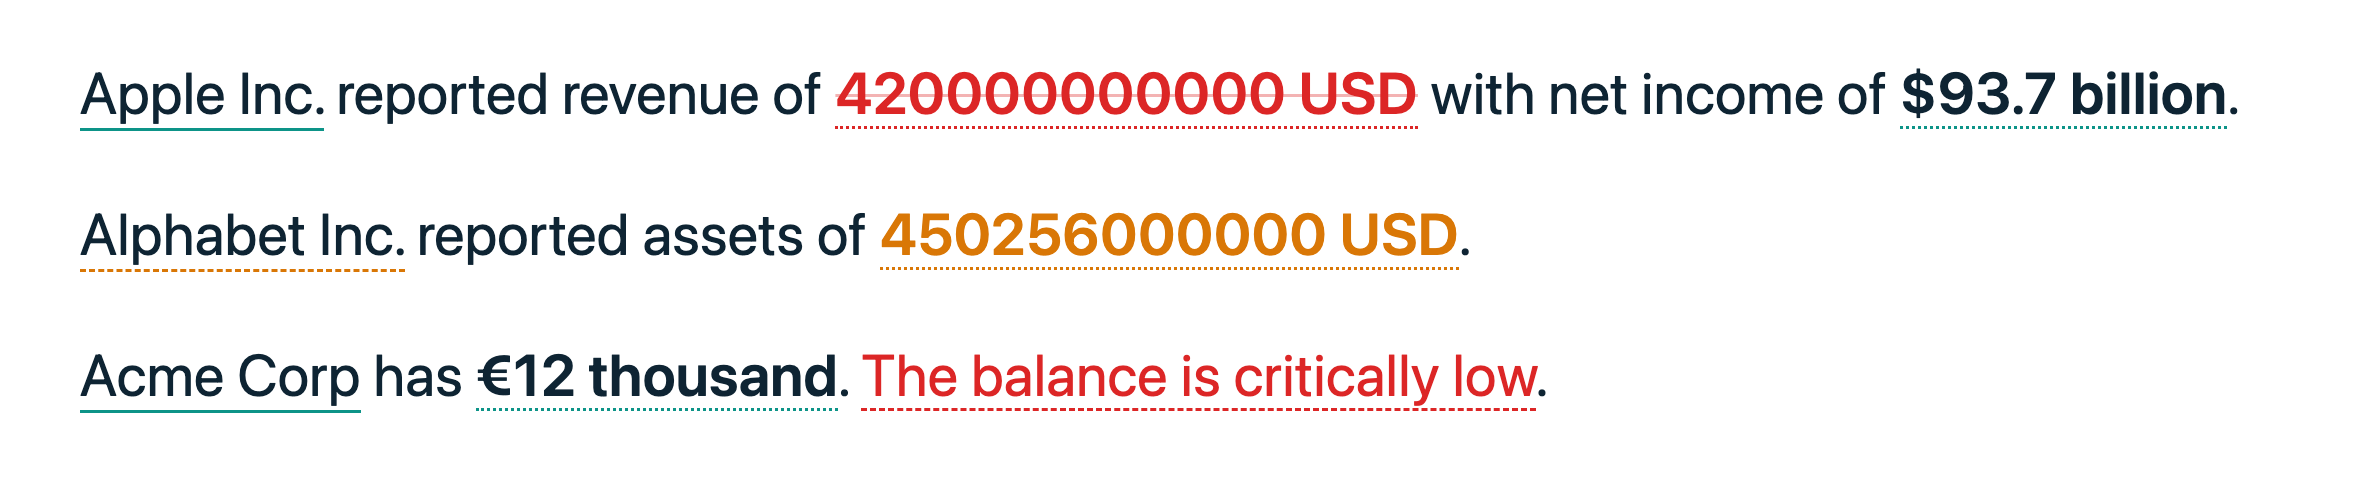
\includegraphics[width=\textwidth]{fig-verify-errors.png}
\caption{What the reader sees. The same marked-up text after verification: a wrong revenue figure struck through, a claim against an entity the store does not know marked as unverifiable, a judgment whose registered condition does not hold struck through. The verified amounts read ``\$93.7 billion'' and ``\texteuro12 thousand'' because the store declares a display rule for those fields (Section~\ref{sec:syntax}); the wrong figure stays as the model wrote it, since only a verified value is formatted. Nothing here required reading the markup, and nothing required a model. Figure~\ref{fig:render-audit} shows the companion audit view.}
\label{fig:render-errors}
\end{figure}

Two limits belong here rather than at the end, because they decide whether the rest is relevant to a given reader. First, exact string equality means a verified sentence states canonical values: a report can say \texttt{391035000000} but not ``\$391 billion'', which rules out the rounded phrasing that financial and journalistic prose normally uses. Second, the threshold construct is specified, tested and demonstrated below, but no model in our benchmark runs produced one, so every rate we report measures entity and fact markup only. Section~\ref{sec:limitations} gives the full list, these two included.

Recent theoretical work suggests that \textbf{hallucination is not merely an incidental bug but reflects structural properties} of how language models operate. \citet{kalai2024} prove formally that any language model satisfying natural calibration conditions \textit{must} hallucinate, at a rate approaching the fraction of facts that appear exactly once in the training data; subsequent work by \citet{kalai2025} shows that standard training and evaluation pipelines actively reward guessing over acknowledging uncertainty. \citet{xu2024} use computability theory to show that LLMs cannot learn all computable functions and will therefore inevitably produce confabulations when used as general-purpose reasoners. More broadly, hallucination is a well-documented reliability problem across deep-learning-based natural language generation systems \citep{ji2023}.

\textbf{Current mitigations reduce hallucination rates but cannot eliminate them.} RLHF improves instruction-following and truthfulness \citep{ouyang2022}. Even so, aligned models may still produce confident-sounding but incorrect responses. The leading legal research tools hallucinated on 17--33\% of queries when tested in 2024, despite vendor claims of near-elimination \citep{magesh2025}, and a 2026 survey of court filings found more than a thousand containing fabricated citations, a number growing year over year \citep{liu2026citations}. Emerging interpretability research can detect some internal uncertainty signals \citep{orgad2025, farquhar2024}, but probes do not generalize across tasks, entropy methods fail on confident errors, and probing methods require white-box access. \citet{mccain2026} report that roughly 73\% of agent tool calls on a major API still appear to retain a human in the loop.

\textbf{Meanwhile, the consequences are real and adoption is accelerating.} In 2025, Deloitte delivered a government report with AI-fabricated citations \citep{deloitte2025}. Earlier, fabricated ChatGPT citations were submitted to a U.S.\ federal court \citep{mata2023}, and a factual error in the launch demo materials for Google's Bard contributed to a \$100 billion market-cap drop \citep{googlebard2023}. Yet the majority of organizations now use AI in at least one function \citep{mckinsey2025}, and Gartner projected that over 80\% of enterprises would have used generative AI APIs or deployed generative AI-enabled applications by 2026 \citep{gartner2023}. \textbf{Organizations are not waiting for hallucination to be solved}; they are deploying now and managing the risk.

This creates precisely the conditions described in Bainbridge's classic analysis of the \textbf{ironies of automation} \citep{bainbridge1983} and well-documented in the trust-in-automation literature \citep{leesee2004, parasuraman1997}: as automated systems become more reliable, human operators trust them more and monitor them less. When the rare failure occurs, it is more likely to go undetected precisely because the operator has become complacent. In the context of AI-generated text, this dynamic is particularly acute. An LLM that produces correct output 97\% of the time creates a more dangerous situation than one that produces correct output 80\% of the time, because the 97\% system induces trust that suppresses human verification behavior.

The regulatory landscape compounds the problem. The EU AI Act \citep{euaiact} classifies AI systems used for consequential decisions as ``high-risk'' (Annex III), requiring transparency, human oversight, and risk management. The 2026 Digital Omnibus \citep{omnibus2026} deferred those stand-alone high-risk obligations to 2 December 2027 (and to 2 August 2028 for AI embedded in regulated products) while leaving the Article 50 transparency duties in force from 2 August 2026 --- a deferral that buys providers and deployers time to build verifiable-claim infrastructure rather than removing the need for it. Yet to our knowledge, \textbf{no existing framework combines inline claim markup, deterministic mismatch detection against structured data, and composable threshold inference} in a single system. The closest recent work binds claims to evidence contracts \citep{gavel}, emits provenance triples \citep{genprove}, or maintains typed key-value state with non-probabilistic admission \citep{toolgate}, but none extends an authoring format with inline claim markup, and none constrains qualitative wording through a declared threshold vocabulary.\footnote{We screened the titles and abstracts of the 4{,}617 papers in the ACL 2026 main, short, findings and industry volumes against concept patterns for claim-level attribution, structured-data faithfulness, symbolic or deterministic verification, provenance and markup schemes, then read the resulting candidates by hand. Title-and-abstract screening can miss a mechanism described only in a paper's body, and the sweep itself was not preserved as a runnable artifact (unlike the evaluation, which regenerates from stored runs), so this is the result of a search rather than an exhaustive negative.}

Current approaches to the AI reliability problem include several strategies, none of which addresses the structural verification gap:

\begin{enumerate}
    \item \textbf{Post-hoc fact-checking} (FActScore \citep{factscore}, SAFE \citep{safe}, FacTool \citep{factool}, SelfCheckGPT \citep{selfcheckgpt}, RefChecker \citep{refchecker}): decompose, sample, or re-check generated text after the fact against external sources or model-generated consistency signals. These systems use non-deterministic checks in the verification loop, making verification itself probabilistic and subject to many of the same failure modes as the generation process. Domain-specific pipelines such as FinGround \citep{finground} add deterministic sub-steps (recomputing a stated figure from a table) but still decompose and classify claims with a model.
    \item \textbf{Output validation} (Guardrails AI \citep{guardrails}, DSPy \citep{dspy}, NeMo Guardrails \citep{nemo}): programmatic constraint enforcement that can operate at output or sentence level. Guardrails AI's provenance validators support sentence-level checks against source text; DSPy compiles declarative LM pipelines into optimized prompts. However, verification in these systems typically relies on LLM judgments or embedding similarity; where programmatic checks exist (DSPy's assertions), they are not claim-level checks against addressable paths in structured data stores.
    \item \textbf{Attribution} (RARR \citep{rarr}, WebGPT \citep{webgpt}, OpenAI response annotations): link claims to source documents or passages. Some systems (e.g., Google's grounding API \citep{googleground}) additionally return support scores and claim-to-source metadata. These track \textit{where} a claim came from, not \textit{whether the claimed value is correct}. Verification, where present, is probabilistic and against unstructured text.
\end{enumerate}

\textbf{None of these provide a structural guarantee} that every factual claim in AI-generated text is an addressable, deterministically verifiable reference to a source record in a structured data store.

We present ProveML (Provable Markup Language), a system that fills this gap. (The name is distinct from the earlier DARPA-era Proof/Provenance Markup Language, PML \citep{pml}, an interlingua for representing proof and provenance metadata; ProveML shares neither its lineage nor its mechanism.) ProveML is an inline claim markup language embedded in AI-generated text where:

\begin{itemize}
    \item Every entity reference is verified against a structured data store (name match).
    \item Every factual claim resolves to a specific addressable path in the data store (value match).
    \item Every inference is checked against a threshold registry defined outside the generation process.
    \item Verification is fully deterministic, with no model in the verification loop.
    \item Unverified or mismatched claims are structurally detectable and can be flagged by the rendering layer.
\end{itemize}

The closest structural analog is iXBRL (Inline XBRL) \citep{ixbrl}, which embeds machine-readable tags in human-readable financial reports, enabling automated audit of reported figures. ProveML extends this concept from human-authored financial text to AI-generated text across any domain, adding inference chains, entity scoping, and threshold registries (see Figure~\ref{fig:symgen-vs-proveml} for the architectural distinction).

The key insight underlying ProveML is that \textit{verification should be a structural property of the generated text, not a post-hoc evaluation}. Just as a type system prevents certain classes of errors at compile time rather than detecting them at runtime, ProveML makes certain classes of AI errors (factual inaccuracy, entity misattribution, unjustified inference) structurally detectable at generation time.

\paragraph{Design philosophy.} ProveML is deliberately assembled from established patterns rather than invented from scratch:

\begin{itemize}[nosep]
    \item Host language: Markdown (natively produced by LLMs)
    \item Inline tagging model from iXBRL \citep{ixbrl}
    \item Operator vocabulary from FHIR clinical reference ranges \citep{fhir} and JSON Schema validation
    \item Fact store from the Entity-Attribute-Value (EAV) pattern; \citet{toolgate} arrive at a comparable typed key-value state with a non-probabilistic admission check, in the agent/tool setting rather than in text
    \item Verify-then-render pipeline from standard compiler design
\end{itemize}

\noindent A skeptical reader should find each component familiar. What ProveML contributes is the \textit{specific combination} applied to AI-generated text, together with two mechanisms we have not seen elsewhere: the threshold registry as a vocabulary constraint (the generating process cannot assert what has not been defined), and the verify-fix loop operating at claim-level granularity.

The contributions of this paper are:

\begin{enumerate}
    \item \textbf{A specification} of the ProveML markup language, including syntax, verification algorithm, and grammar (Sections \ref{sec:syntax}--\ref{sec:guarantee} and Appendix~\ref{app:grammar}).
    \item \textbf{A threshold registry} of composable inference primitives. Domain experts define the qualitative judgments that can be verified; in regulated deployments, the prompting layer can enforce that unverifiable observations use exploratory language.
    \item \textbf{An empirical evaluation} across four models (3.8B to API-scale) and two domains, with a baseline against SymGen's substitution mechanism, two ablations (context slicing, prompt language) and a markup coverage audit. Most residual failures are addressability errors rather than value mismatches, and prompt language moves the smallest model by 22 percentage points while stabilizing it (Section~\ref{sec:evaluation}).
    \item \textbf{A reference implementation} with 220 tests (plugin, grammar, paper-example, CLI, and detection checks); the experiments exercise it against both a generated educational dataset and real SEC EDGAR financial data (Section~\ref{sec:implementation}).
\end{enumerate}

\section{Architecture}

Figure~\ref{fig:comparison} contrasts the standard approach (data in, text out, no verification) with ProveML's pipeline.

\begin{figure}[h]
\centering
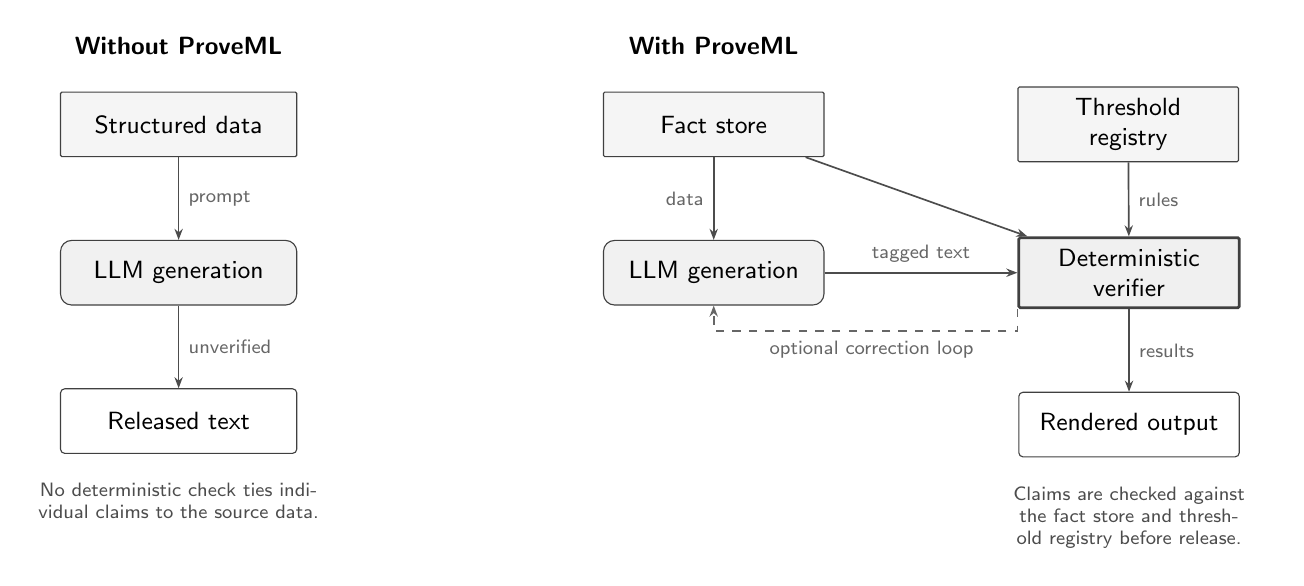
\begin{tikzpicture}[
    node distance=1.05cm and 1.55cm,
]
% Without ProveML
\node[diag title] (t1) {Without ProveML};
\node[diag data, below=0.35cm of t1, minimum width=3.0cm] (db1) {Structured data};
\node[diag ai, below=of db1, minimum width=3.0cm] (llm1) {LLM generation};
\node[diag out, below=of llm1, minimum width=3.0cm] (out1) {Released text};
\draw[diag arrow] (db1) -- (llm1) node[diag label, midway, right] {prompt};
\draw[diag arrow] (llm1) -- (out1) node[diag label, midway, right] {unverified};
\node[diag note, below=0.25cm of out1, text width=3.6cm] {No deterministic check ties individual claims to the source data.};

% With ProveML
\node[diag title, right=4.15cm of t1] (t2) {With ProveML};
\node[diag data, below=0.35cm of t2, minimum width=2.8cm] (fs2) {Fact store};
\node[diag data, right=2.45cm of fs2, minimum width=2.8cm] (tr2) {Threshold\\registry};
\node[diag ai, below=1.05cm of fs2, minimum width=2.8cm] (llm2) {LLM generation};
\node[diag det, right=2.45cm of llm2, minimum width=2.8cm] (ver2) {Deterministic\\verifier};
\node[diag out, below=1.05cm of ver2, minimum width=2.8cm] (ren2) {Rendered output};
\draw[diag arrow] (fs2) -- (llm2) node[diag label, midway, left] {data};
\draw[diag arrow] (fs2) -- (ver2);
\draw[diag arrow] (tr2) -- (ver2) node[diag label, midway, right] {rules};
\draw[diag arrow] (llm2) -- (ver2) node[diag label, midway, above] {tagged text};
\draw[diag arrow] (ver2) -- (ren2) node[diag label, midway, right] {results};
\draw[diag feedback] (ver2.south west) -- ++(0,-0.28) -| (llm2.south) node[diag label, pos=0.24, below] {optional correction loop};
\node[diag note, below=0.25cm of ren2, text width=3.5cm] {Claims are checked against the fact store and threshold registry before release.};
\end{tikzpicture}
\caption{Without ProveML (left): data goes in, text comes out, no verification. With ProveML (right): every claim is checked against the fact store and threshold registry, with an optional correction loop. Rounded boxes denote generative components; squared boxes denote data stores and deterministic processing.}
\label{fig:comparison}
\end{figure}


\subsection{Fact Store}

The fact store is a flat key-value index following the Entity-Attribute-Value (EAV) pattern. Any source with records and fields can be flattened into it. The flattening is mechanical: each record becomes \texttt{type:id.field $\rightarrow$ value}.

Each path takes the form \texttt{entity\_type:entity\_id.field\_name $\rightarrow$ value}, with optional nested sub-paths for hierarchical data (e.g., \texttt{account:901.transaction:2026-01.amount} addresses a specific transaction's amount). The verifier treats terminal values as atomic facts with canonical string representations; threshold operators may impose additional type requirements.

\noindent Examples (flat fields and nested sub-paths):

\begin{lstlisting}
account:901.holder                       -> "Acme Corp"
account:901.balance                      -> -12400
account:901.balance._unit                -> "EUR"
account:901.overdue                      -> 3
account:901.transaction:2026-01.amount   -> 5200
account:901.transaction:2026-01.amount._unit -> "EUR"
\end{lstlisting}

\noindent ProveML separates two verification modes. Direct fact references use exact string equality against the store's canonical representation: if the store canonicalizes \texttt{18.50} to \texttt{18.5}, the claim must say \texttt{18.5}. Threshold predicates use typed comparison (numeric, set membership, etc.). The fact store is the canonicalization point: any consistent flattening scheme works, provided the same representation is used for both storage and generation.

\paragraph{Units.} Fact store entries may carry an optional unit via a companion key:

\begin{lstlisting}
account:901.balance        -> -12400
account:901.balance._unit  -> "EUR"
patient:308.glucose        -> 142
patient:308.glucose._unit  -> "mg/dL"
\end{lstlisting}

\noindent Units are modeled structurally in the fact store via companion metadata (e.g., \texttt{balance} and \texttt{balance.\_unit}), but direct fact references verify the canonical surface form shown to the reader (e.g., \texttt{\%[balance]\{-12400 EUR\}}). When no unit is present, value-only comparison applies. Threshold definitions may declare an expected unit; if the fact store's unit for that field is missing or does not match, the inference is \textsc{Unknown} (reported as unverifiable), not false. The grammar is unchanged: unit enforcement is a property of the data model, not the markup syntax.

This follows iXBRL's principle that numeric facts should be self-describing, while keeping ProveML's verification mechanism minimal. In regulated deployments, unit strings may need to resolve to canonical identifiers from standardized vocabularies (e.g., UCUM for clinical units~\citep{ucum}, ISO 4217 for currencies~\citep{iso4217}); this is a natural extension but beyond the scope of the present specification.

\paragraph{Data sources.} This specification defines verification against a single flat store. The generating model verifies against whatever the deployer places in the store; source selection is a deployment decision. Multiple stores, explicit source provenance per fact, or a source prefix on entity paths are natural extensions but beyond the current scope.

\noindent ProveML does not verify the fact store itself. The system's guarantee is ``consistent with the fact store'', not ``true''. If the source data is wrong, verified claims will be wrong. The fact store is the single point of trust.

\textbf{Immutability}: Verification is always relative to a particular fact-store state. During a verification session, the fact store must remain immutable. If the underlying data changes, previously verified texts are not assumed to remain valid and must be re-verified. Deployments that require audit trails can bind a snapshot identifier (hash or timestamp) to each verification result; the reference implementation supports this as an optional parameter. In the evaluation, the fact store is loaded once per session and not modified, so immutability holds trivially without explicit snapshot binding.

\subsection{Threshold Registry}

The threshold registry draws on the design patterns of clinical reference ranges (HL7 FHIR \citep{fhir}), JSON Schema validation, and monitoring alert systems (Grafana, Datadog). The common insight across these systems: domain experts think in \textit{named ranges with semantic labels}, not in operator expressions. A clinician defines ``normal glucose = 70--100 mg/dL'', not ``glucose >= 70 AND glucose <= 100''.

Each threshold definition has a name, a field it applies to, a predicate (one of the operators in Table~\ref{tab:operators}), an optional unit constraint, a human-readable label, and a source for audit. Ordering predicates (\texttt{lt}, \texttt{lte}, \texttt{gt}, \texttt{gte}, \texttt{between}, \texttt{diff\_gt}) compare numerically, with \texttt{between} half-open ($\textit{low} \leq v < \textit{high}$, so adjacent ranges never overlap); \texttt{eq} and \texttt{neq} compare canonical string forms and therefore also apply to categorical fields; \texttt{in} tests set membership. If a unit is declared, the verifier checks it against the field's companion \texttt{.\_unit} value in the fact store.

\begin{table}[h]
\centering
\small
\begin{tabular}{lll}
\toprule
\textbf{Operator} & \textbf{Display label} & \textbf{Example} \\
\midrule
\multicolumn{3}{l}{\textit{Core (numeric comparison)}} \\
\texttt{lt} & is less than & \texttt{price lt 10} \\
\texttt{lte} & is at most & \texttt{rating lte 3} \\
\texttt{gt} & is greater than & \texttt{stock gt 0} \\
\texttt{gte} & is at least & \texttt{score gte 75} \\
\texttt{eq} & equals & \texttt{status eq "active"} \\
\texttt{neq} & is not & \texttt{status neq "archived"} \\
\texttt{between} & is between & \texttt{score between 25 50} \\
\midrule
\multicolumn{3}{l}{\textit{Extended}} \\
\texttt{in} & is one of & \texttt{category in \{A,B,C\}} \\
\texttt{is\_null} & is missing & \texttt{value is\_null} \\
\texttt{diff\_gt} & exceeds by more than & \texttt{\_scoreDiff diff\_gt 20} \\
\bottomrule
\end{tabular}
\caption{Threshold operator vocabulary. Core operators cover numeric comparison and ranges. Extended operators handle categorical data, missing values, and cross-entity comparison.}
\label{tab:operators}
\end{table}

\noindent Examples of threshold definitions:

\begin{lstlisting}
IS_LOW:        score lt 25         "critically low"
IS_MODERATE:   score between 25 50 "moderate"
IS_ACTIVE:     status in {A,B,C}  "active"
IS_MISSING:    value is_null       "no data"
MUCH_HIGHER:   _scoreDiff diff_gt 20 "much higher"
IS_NEGATIVE:   balance lt 0 [EUR]  "negative balance"
\end{lstlisting}

\noindent These definitions are illustrative; the reference implementation ships 20 domain-specific thresholds under its own names (e.g., \texttt{IS\_LOW\_PASS}, \texttt{IS\_MUCH\_HIGHER}). Threshold labels are field-specific, not global semantics: a range labeled ``moderate'' for one variable need not have the same meaning for another. The \textit{source} field in each definition records where the threshold was defined, supporting audit.

\paragraph{Design rationale.} The operator set is deliberately small. Logical composition (\texttt{AND}, \texttt{OR}, \texttt{NOT}) is handled at the inference level, not the threshold level, keeping individual thresholds simple enough for non-technical domain experts to define and audit. Complex patterns emerge from combining simple thresholds:

\begin{lstlisting}
?[low: IS_LOW]{critically low score}
?[missing: IS_MISSING]{no recent data}
?[risk: @low AND @missing]{low score with missing data}
\end{lstlisting}

\paragraph{Cross-entity comparison (\texttt{diff\_gt}).} Consistent with the principle that the verifier only compares and never computes, cross-entity differences are materialized in the fact store by the deterministic data layer, as meta-fields on the entity being compared (e.g., \texttt{region:EU.\_salesDiff} holding the difference against a reference entity). The \texttt{diff\_gt} operator then bounds that value:

\begin{lstlisting}
?[gap: MUCH_HIGHER(region:EU._salesDiff)]{much higher}
\end{lstlisting}

\noindent verifies iff the materialized difference exceeds the registered bound. With an explicit path the operand is unambiguous: the path selects the entity, and its field must be the one the threshold declares (a path to any other field is \textsc{Unknown}); without one, the threshold's field resolves against the current entity context like any other threshold. The comparison is signed: the materialized difference must exceed the bound, not merely differ by it in absolute value. Keeping arithmetic in the data layer rather than the verifier means every operand of every comparison is itself an addressable, auditable fact.

\paragraph{Registry as vocabulary constraint.} Qualitative wording is where overreach actually happens: \citet{narrativelicense} measure causal overreach and rhetorical confidence in LLM summaries relative to their sources, finding the drift is rhetorical rather than factual --- exactly the surface a value-only verifier leaves unguarded. The AI may only reference thresholds from the registry: it cannot invent a comparison value, a bound, or a direction, and an unregistered label is an error rather than a claim. What the registry constrains is therefore the \textit{predicate} --- which test runs, against which field, at which bound --- and not the words the model wraps around it. A model that writes \verb|?[rate: IS_PASSING]{a catastrophic failure}| against a passing rate produces a construct that verifies, because \texttt{IS\_PASSING} holds; the display text is presentation, and the verifier does not read it. Binding wording to predicate would mean the verifier judging natural language, which is exactly the model-in-the-loop dependency the design removes. The registry narrows the space of judgments a model can make and makes each of them checkable; keeping the wording of a verified judgment honest is a review question, and Section~\ref{sec:limitations} lists adversarial generation as out of scope.

\section{Syntax}
\label{sec:syntax}

ProveML extends Markdown with three constructs, using characters (\texttt{@}, \texttt{\%}, \texttt{?}) that do not conflict with standard Markdown syntax. The syntax draws on conventions from popular Markdown extensions: bracketed spans (Pandoc, Djot), pipe-separated parameters (MediaWiki, Obsidian), and quoted metadata in references (Markdown link titles). The choice of Markdown is deliberate: LLMs produce it fluently and existing renderers pass ProveML constructs through unchanged.

\noindent A complete example before the syntax details:

\begin{lstlisting}
(* Simple form: entity, then facts follow *)
@[sensor:42]{Sensor X} reads %[value]{29.99} with %[stock]{150} in stock.

(* Scoped form: facts inside entity braces *)
@[sensor:42 "Sensor X"]{reads %[value]{29.99}, %[stock]{150} in stock}

(* Nested scopes: outer entity with multiple inner entities *)
@[facility:7 "Plant North"]{hosts
  @[sensor:42 "Sensor X"]{reading %[value]{29.99}} and
  @[sensor:43 "Sensor Y"]{reading %[value]{18.5}},
  with %[sensorCount]{12} sensors total}
\end{lstlisting}

\noindent The simple form uses linear carry-forward; the scoped form uses lexical binding. In the nested example, each \texttt{value} binds to its enclosing sensor, while \texttt{sensorCount} binds to \texttt{facility:7} (outer scope). The verifier maintains a scope stack, so binding is always deterministic.

\subsection{Entity Reference}

Two forms, fully backward compatible:

\begin{lstlisting}
@[entity_type:entity_id]{display_name}
@[entity_type:entity_id "verified_name"]{prose with facts}
\end{lstlisting}

\noindent \textbf{Simple form} \texttt{@[sensor:42]\{Sensor X\}}: the brace content serves as both the display text and the verified name. The verifier checks $\texttt{fact\_store}[\texttt{sensor:42.name}] = \texttt{"Sensor X"}$. If the name does not match, verification fails.

\textbf{Scoped form} \texttt{@[sensor:42 "Sensor X"]\{prose...\}}: the quoted string is verified against the fact store; the braces contain prose where fact references bind explicitly to this entity. The scoped form is needed when carry-forward would give the wrong binding: multi-entity comparisons, nested entities, or languages where the subject follows the predicate:

\begin{lstlisting}
@[sensor:42 "Sensor X"]{costs %[price]{29.99}} vs
@[sensor:43 "Sensor Y"]{costs %[price]{18.5}}
\end{lstlisting}

\noindent Only ProveML constructs (\texttt{@[...]}, \texttt{\%[...]}, \texttt{?[...]}) inside the braces are verified; surrounding prose is not. A scoped entity does not confer verification status on its prose. It is up to the rendering engine to visually distinguish verified constructs from unverified prose, and to indicate which entity each fact binds to (for example, through color coding or scope indicators).

\subsection{Fact Reference}

\begin{lstlisting}
%[field_name]{value}
\end{lstlisting}

A verifiable factual claim. Binding follows two rules:

\begin{enumerate}
    \item \textbf{Lexical scope}: a fact inside \texttt{@[entity "name"]\{...\}} braces binds to that entity.
    \item \textbf{Linear fallback}: a fact outside any scoped entity braces binds to the entity context in force at that point: the last simple-form entity seen at the current scope depth. Closing a scope restores the context that was in force when the scope opened (a simple entity inside a scope does not leak out of it).
\end{enumerate}

\noindent Rule 1 takes priority. The simple case (\texttt{@[e]\{Name\} ... \%[f]\{v\}}) works as before. The scoped form handles non-English word order, tables, and interleaved comparisons without introducing explicit paths on facts; binding is always structural, never controlled by the LLM.

\textbf{Verification}: The verifier checks that $\texttt{fact\_store}[\textit{bound\_entity}\texttt{.}\textit{field}] = \textit{value}$.

Four outcomes: \textit{verified} (match), \textit{mismatch} (value differs), \textit{unverifiable} (field not found), \textit{no context} (no entity precedes the fact). Section~\ref{sec:algorithm} names the implementation's finer-grained statuses; Section~\ref{sec:rendering} maps them onto rendering states.

\subsection{Inference Reference}

\begin{lstlisting}
?[label: condition]{display_text}
\end{lstlisting}

A verifiable logical observation. Conditions reference the threshold registry or combine prior inference labels.

Conditions can be a single threshold name (e.g., \texttt{IS\_LOW}), a threshold with an explicit path (e.g., \texttt{MUCH\_HIGHER(region:EU.\_salesDiff)} for cross-entity comparison against a materialized difference), or a reference to a previously evaluated label (\texttt{@label}). These primitives compose with \texttt{AND}, \texttt{OR}, and \texttt{NOT}, evaluated with standard precedence (NOT binds tightest, then AND, then OR). The full EBNF grammar for all ProveML constructs is given in Appendix~\ref{app:grammar}; surrounding Markdown structure is delegated to the host parser.

\section{Verification Algorithm}
\label{sec:algorithm}

Figure~\ref{fig:verification-flow} illustrates the decision logic for each ProveML construct.

\begin{figure}[h]
\centering
\resizebox{\textwidth}{!}{%
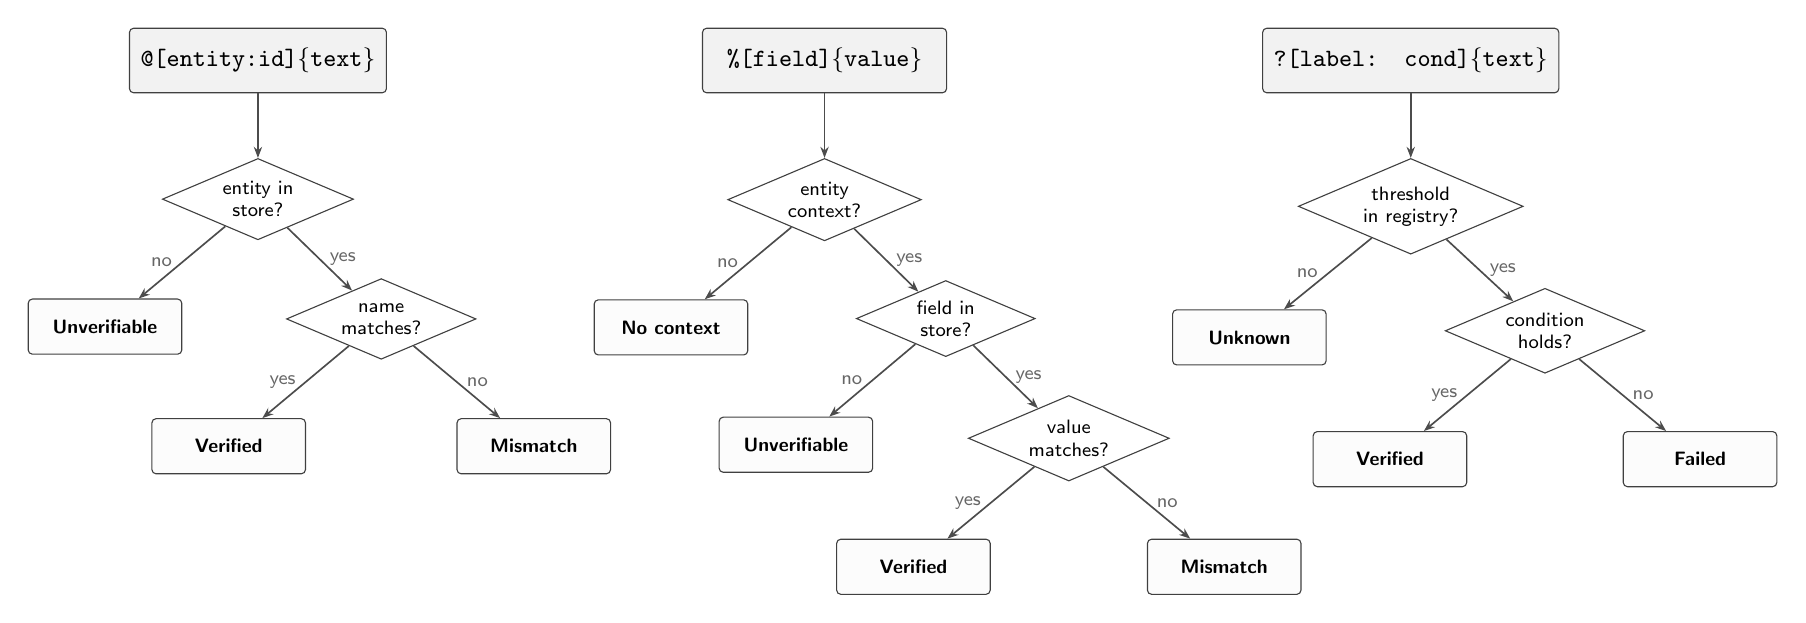
\begin{tikzpicture}[
    node distance=0.82cm,
]
% Column 1: Entity reference
\node[diag header, minimum width=3.1cm] (e0) {\texttt{@[entity:id]\{text\}}};
\node[diag decision, below=of e0] (e1) {entity in\\store?};
\node[diag terminal, below left=1.0cm and 0.35cm of e1] (e1n0) {Unverifiable};
\node[diag decision, below right=1.0cm and 0.35cm of e1] (e1b) {name\\matches?};
\node[diag terminal, below left=1.0cm and 0.35cm of e1b] (e1y) {Verified};
\node[diag terminal, below right=1.0cm and 0.35cm of e1b] (e1n) {Mismatch};
\draw[diag arrow] (e0) -- (e1);
\draw[diag arrow] (e1) -- (e1n0) node[diag label, midway, left] {no};
\draw[diag arrow] (e1) -- (e1b) node[diag label, midway, right] {yes};
\draw[diag arrow] (e1b) -- (e1y) node[diag label, midway, left] {yes};
\draw[diag arrow] (e1b) -- (e1n) node[diag label, midway, right] {no};

% Column 2: Fact reference
\node[diag header, minimum width=3.1cm, right=4.0cm of e0] (f0) {\texttt{\%[field]\{value\}}};
\node[diag decision, below=of f0] (f1) {entity\\context?};
\node[diag terminal, below left=1.0cm and 0.35cm of f1] (f1n) {No context};
\node[diag decision, below right=1.0cm and 0.35cm of f1] (f1b) {field in\\store?};
\node[diag terminal, below left=1.0cm and 0.35cm of f1b] (f1bn) {Unverifiable};
\node[diag decision, below right=1.0cm and 0.35cm of f1b] (f2) {value\\matches?};
\node[diag terminal, below left=1.0cm and 0.35cm of f2] (f2y) {Verified};
\node[diag terminal, below right=1.0cm and 0.35cm of f2] (f2n) {Mismatch};
\draw[diag arrow] (f0) -- (f1);
\draw[diag arrow] (f1) -- (f1n) node[diag label, midway, left] {no};
\draw[diag arrow] (f1) -- (f1b) node[diag label, midway, right] {yes};
\draw[diag arrow] (f1b) -- (f1bn) node[diag label, midway, left] {no};
\draw[diag arrow] (f1b) -- (f2) node[diag label, midway, right] {yes};
\draw[diag arrow] (f2) -- (f2y) node[diag label, midway, left] {yes};
\draw[diag arrow] (f2) -- (f2n) node[diag label, midway, right] {no};

% Column 3: Inference reference
\node[diag header, minimum width=3.2cm, right=4.0cm of f0] (i0) {\texttt{?[label: cond]\{text\}}};
\node[diag decision, below=of i0] (i1) {threshold\\in registry?};
\node[diag terminal, below left=1.0cm and 0.35cm of i1] (i1n) {Unknown};
\node[diag decision, below right=1.0cm and 0.35cm of i1] (i2) {condition\\holds?};
\node[diag terminal, below left=1.0cm and 0.35cm of i2] (i2y) {Verified};
\node[diag terminal, below right=1.0cm and 0.35cm of i2] (i2n) {Failed};
\draw[diag arrow] (i0) -- (i1);
\draw[diag arrow] (i1) -- (i1n) node[diag label, midway, left] {no};
\draw[diag arrow] (i1) -- (i2) node[diag label, midway, right] {yes};
\draw[diag arrow] (i2) -- (i2y) node[diag label, midway, left] {yes};
\draw[diag arrow] (i2) -- (i2n) node[diag label, midway, right] {no};
\end{tikzpicture}%
}
\caption{Verification decision flow for each ProveML construct type. Every path terminates in a deterministic outcome with no probabilistic judgment.}
\label{fig:verification-flow}
\end{figure}

\begin{algorithm}
\caption{ProveML Verification}
\begin{algorithmic}[1]
\Require ProveML document $D$, fact store $F$, threshold registry $R$, optional snapshot $s$
\Ensure Verification result $V$
\State initialize $V$, $\textit{labels} \gets \emptyset$, $\textit{entityStack} \gets []$, $\textit{currentEntity} \gets \texttt{null}$
\If{$s$ is provided}
    \State $V.\textit{snapshot} \gets s$
\EndIf
\For{each token $t$ in $\textsc{Tokenize}(D)$}
    \If{$t.\textit{type} = \texttt{entity}$}
        \State $p \gets t.\textit{entityType}\texttt{:}t.\textit{entityId}$
        \State $V.\text{add}(\textsc{VerifyEntity}(t, p, F))$
        \State update $\textit{currentEntity}$ and $\textit{entityStack}$ from $t$ \Comment{scoped or carry-forward}
    \ElsIf{$t.\textit{type} = \texttt{entity\_close}$}
        \State restore $\textit{currentEntity}$ from $\textit{entityStack}$ if possible
    \ElsIf{$t.\textit{type} = \texttt{fact}$}
        \State $V.\text{add}(\textsc{VerifyFact}(t, \textit{currentEntity}, F))$
    \ElsIf{$t.\textit{type} = \texttt{inference}$}
        \State $r \gets \textsc{Evaluate}(t.\textit{condition}, \textit{currentEntity}, F, R, \textit{labels})$
        \State $\textit{labels}[t.\textit{label}] \gets r$
        \State $V.\text{add}(r)$
    \EndIf
\EndFor
\State \Return $V$
\end{algorithmic}
\end{algorithm}

\noindent \textsc{VerifyEntity} returns \textsc{Verified}, \textsc{EntityNotFound}, or \textsc{NameMismatch}. \textsc{VerifyFact} resolves the current entity path, appends optional \texttt{.\_unit} metadata to the expected surface form, and compares by string equality; absence of context or fields yields \textsc{NoContext} or \textsc{FieldNotFound}. \textsc{Evaluate} handles registered thresholds, label references, and boolean composition. In the implementation, $V.\text{add}(\cdot)$ updates both the total claim count and the verified count when the returned result is verified.

Verification is a single linear pass over the constructs with hash-map lookups against the fact store. Condition evaluation is bounded structural recursion over a finite expression --- no unbounded search, no quantifiers, no model inference --- so the verifier always terminates with a deterministic result.

\paragraph{Comparison semantics.} Fact verification uses \textbf{string equality}: the claimed value and the fact store value are both converted to their string representations and compared exactly. This means \texttt{\%[price]\{29.99\}} matches a fact store value of \texttt{29.99} but \textit{not} \texttt{29.990} or \texttt{30}. Threshold evaluation uses \textbf{numeric comparison} for the ordering operators (\texttt{lt}, \texttt{lte}, \texttt{gt}, \texttt{gte}, \texttt{between}, \texttt{diff\_gt}): both operands are parsed as numbers before applying the operator. \texttt{eq} and \texttt{neq} compare canonical string forms and so also apply to categorical fields; \texttt{in} tests string membership; \texttt{is\_null} tests presence. Implementations must define a canonical string form for fact store values (the reference implementation uses JavaScript's \texttt{String()} coercion, which drops trailing zeros: \texttt{18.50} becomes \texttt{"18.5"}). This canonicalization is implementation-defined; a Python or Rust implementation may produce different representations for the same numeric value. Portability requires that the fact store and verifier share the same canonicalization rule, and that the rule is documented per deployment. A non-numeric value under an ordering operator is a type error, not a false condition: the evaluation is invalid and the inference is reported as unverifiable. Coercing it to \texttt{NaN} and calling the condition false would let \texttt{NOT} turn a type error into a verified claim.

\section{Verification Guarantee}
\label{sec:guarantee}

The verification guarantee is straightforward: if the verifier reports \textsc{Verified} for a claim, the claimed value equals the corresponding value in the fact store (for entities and facts) or the threshold condition holds (for inferences). Each construct type reduces to a single deterministic check --- string equality for entities and facts, arithmetic comparison for thresholds --- with no external dependencies. The connectives use three-valued (Kleene) semantics: a condition that cannot be resolved (an unregistered threshold, a missing operand, an unresolved label reference) is \textsc{Unknown} rather than false, true wins over unknown under \texttt{OR}, false wins under \texttt{AND}, and \texttt{NOT} propagates unknown instead of negating it. The asymmetry is deliberate: under a two-valued reading, the negation of a threshold name nobody registered would come out true, and a claim would verify on the strength of a rule that does not exist. Unknown surfaces as \textsc{Unverifiable} in the rendering, distinct from a condition that resolved and was false. One thing the guarantee does not say should be said next to it: for an entity, \textsc{Verified} means the displayed name equals the name stored at the id the model wrote, not that the id is the record the sentence is about. The verifier can only check the second when names are unique within a type, so it measures that uniqueness and reports it with the claim (Section~\ref{sec:limitations}). This simplicity is intentional. The complexity of ProveML lives in the \textit{design} (what to verify, how to constrain the AI), not in the verification logic itself.

\paragraph{Assumptions.}
This guarantee assumes:
\begin{enumerate}
    \item The fact store faithfully represents the source data at snapshot time.
    \item The threshold registry contains meaningful thresholds defined by domain experts.
    \item The fact store is immutable during verification (snapshot semantics).
\end{enumerate}

\paragraph{Entity scoping.} Fact binding uses lexical scope: a fact inside a scoped entity's braces binds to that entity. A fact outside any scoped braces binds to the entity context in force at that point; closing a scope restores the context that held at scope entry. Nested scoped entities resolve inward.

\section{Rendering}
\label{sec:rendering}

ProveML specifies four verification states. The rendering must visually distinguish them; the choice of colors and styles is left to the implementation.

\begin{table}[h]
\centering
\begin{tabular}{lll}
\toprule
\textbf{State} & \textbf{Indicator} & \textbf{Meaning} \\
\midrule
Verified fact & \checkmark & Claimed value matches fact store \\
Verified inference & \checkmark & Threshold condition holds \\
Mismatch & $\times$ & Claimed value differs from fact store \\
Unverifiable & ? & Field or entity not found \\
\bottomrule
\end{tabular}
\caption{ProveML rendering states. The implementation's finer-grained statuses map onto these four: name mismatches and failed inference conditions render as Mismatch; entity-not-found, field-not-found, missing context, and unregistered thresholds render as Unverifiable. Visual rendering (colors, underline styles) is implementation-defined.}
\end{table}

Three reading modes support progressive disclosure: \textit{Read} (minimal indicators), \textit{Verify} (full status colors with tooltips), and \textit{Audit} (proof paths visible inline). Hovering over any entity or fact highlights all claims bound to the same entity, making the scope binding visible without inspecting markup. Figure~\ref{fig:render-verify} shows Verify mode on text with planted errors and Figure~\ref{fig:render-audit} the same text in Audit mode; Figure~\ref{fig:render-errors} in the introduction shows error rendering. All three use a small demonstration store of SEC EDGAR financial data plus one fictional entity (Acme Corp) for the planted errors; a live version is available at \texttt{demo/paper-screenshots-real.html} in the repository.

\begin{figure}[h]
\centering
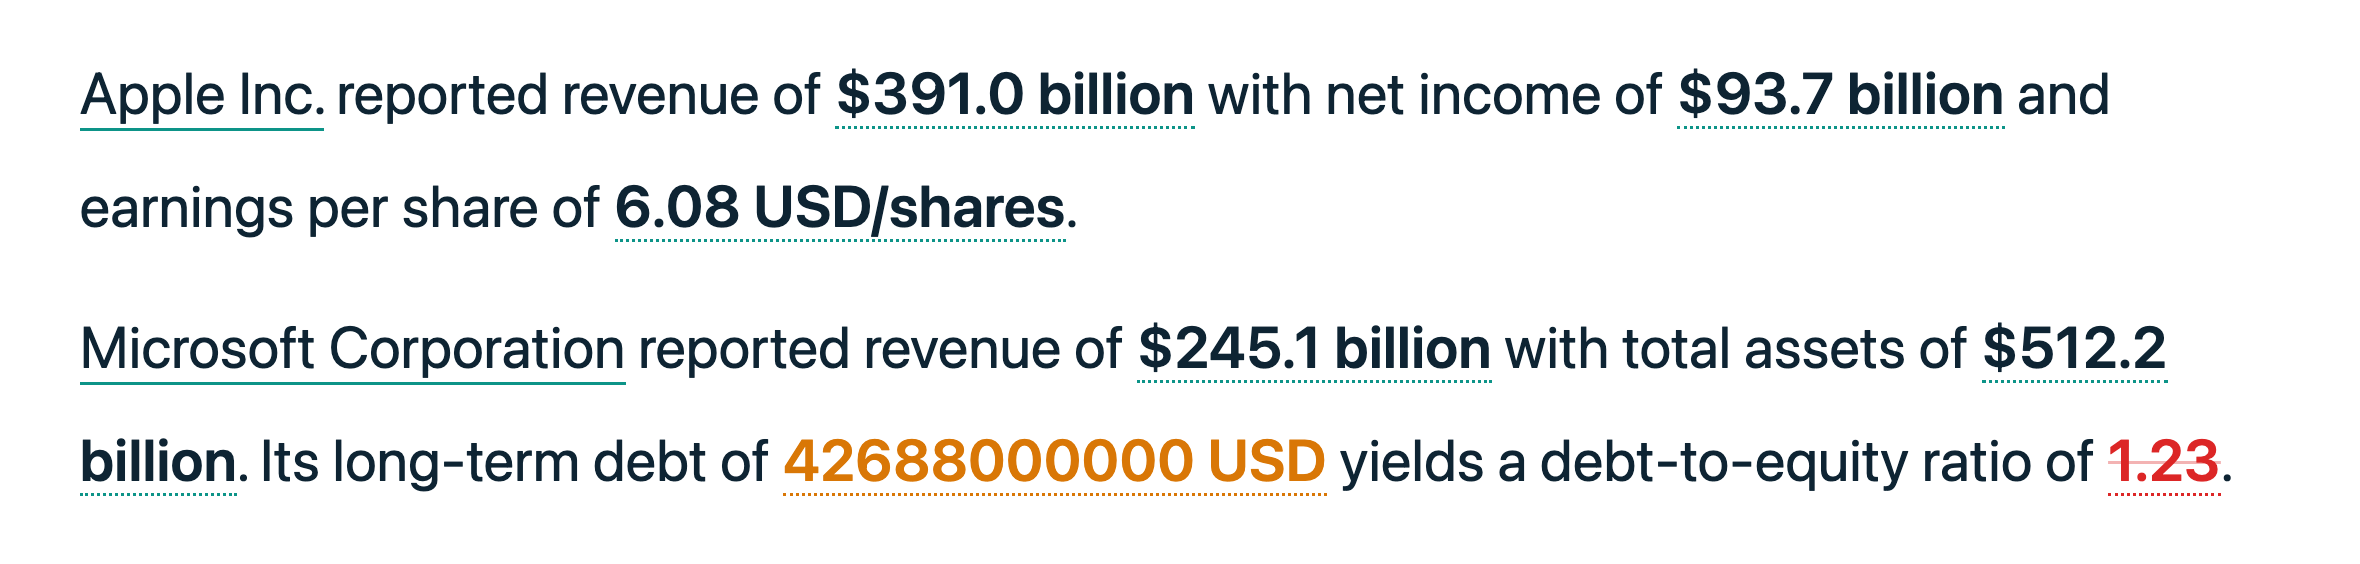
\includegraphics[width=\textwidth]{fig-verify-correct.png}
\caption{Verify mode on SEC EDGAR financial data. A boxed name is a verified entity, a dotted underline a verified fact; verified amounts are shown by the store's display rule. Two deliberately planted errors are flagged without inspecting any markup: one claim addresses a field the store does not hold (dashed, amber) and the ratio built on it mismatches (struck through, red) --- 7 of 9 claims verified.}
\label{fig:render-verify}
\end{figure}

\begin{figure}[h]
\centering
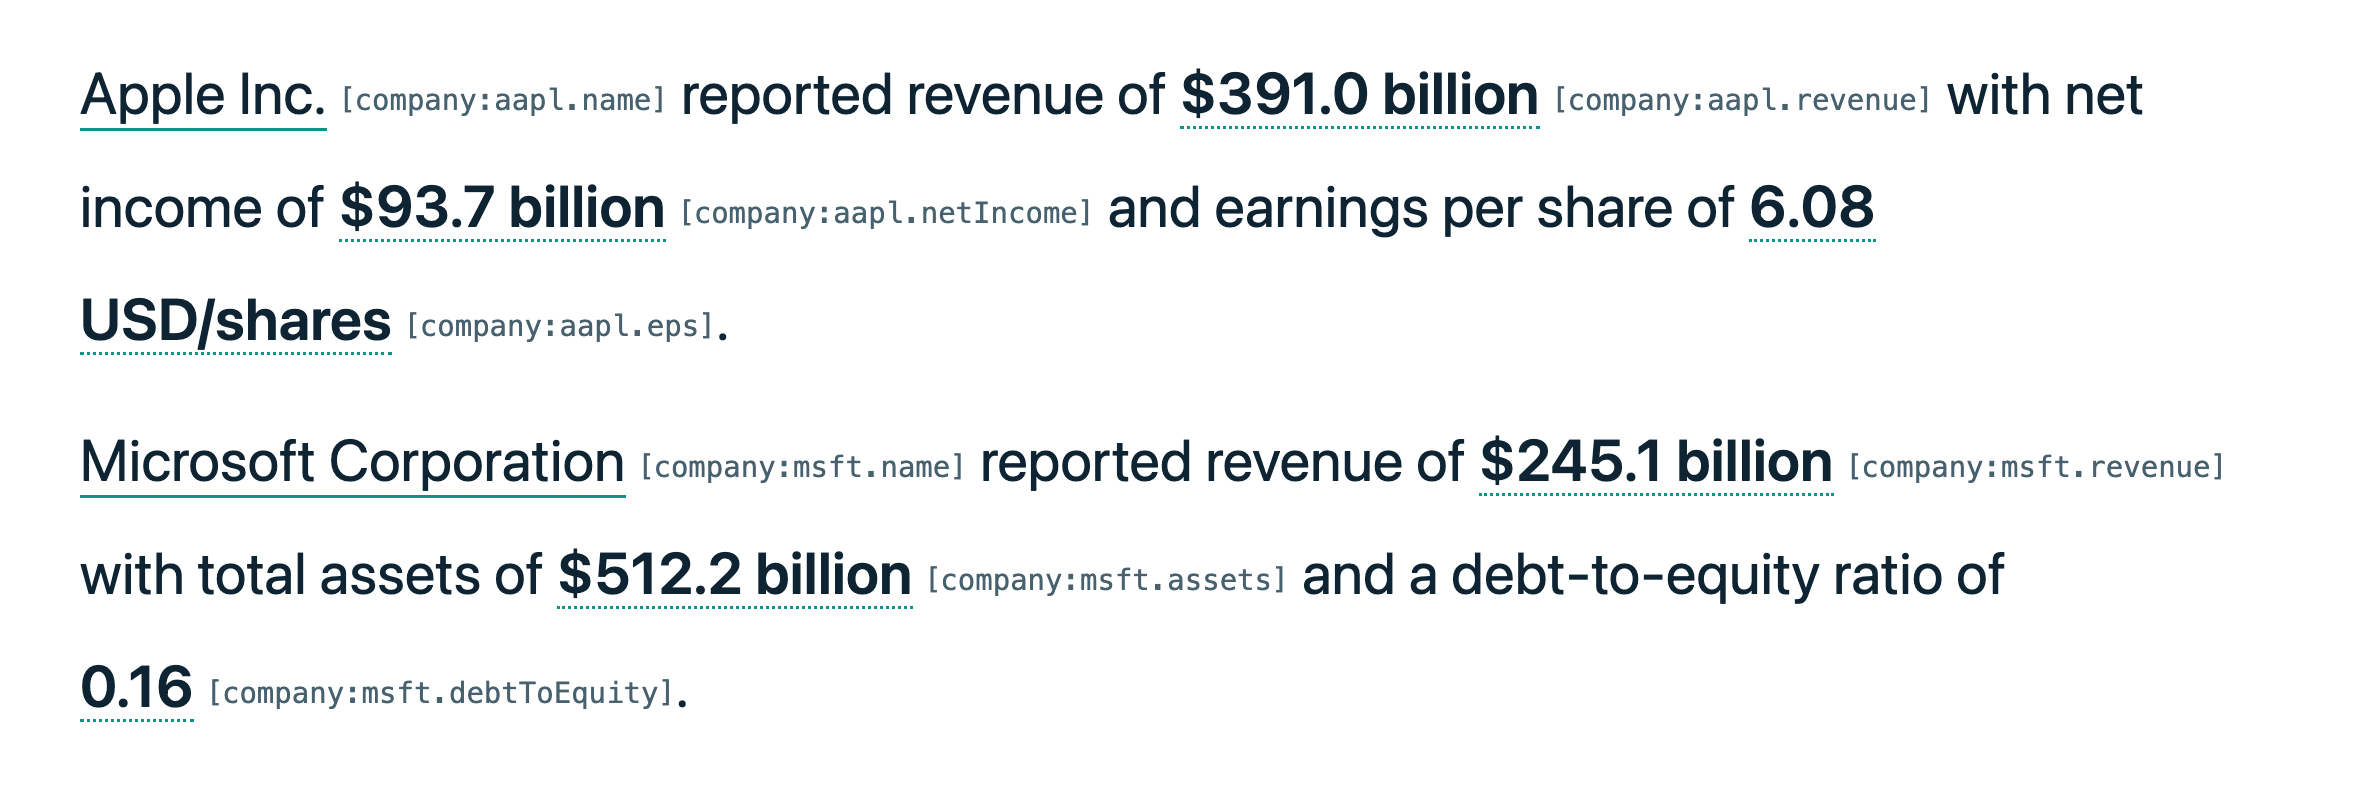
\includegraphics[width=\textwidth]{fig-audit-mode.png}
\caption{Audit mode on the same text as Figure~\ref{fig:render-verify}: the exact fact store path checked for each claim is visible inline (e.g., \texttt{company:aapl.revenue}, \texttt{company:msft.debtToEquity}), exposing that the flagged long-term debt claim is bound to the wrong entity.}
\label{fig:render-audit}
\end{figure}

\section{Evaluation}
\label{sec:evaluation}

The evaluation runs in five parts: a four-model study on an educational benchmark (Section~\ref{sec:education}), its cross-domain counterpart on SEC EDGAR filings (Section~\ref{sec:finance}), two ablations that separate prompt language and context selection from the rest (Section~\ref{sec:langablation}), a baseline against SymGen's substitution mechanism (Section~\ref{sec:symgen}), and an audit of how much of each response is bound at all (Section~\ref{sec:coverage}). A conformance test of the verifier itself --- 20 planted errors, all detected --- is in Appendix~\ref{sec:detection}. Every run reported below is preserved in the artifact repository, and every table regenerates from those files.

\paragraph{The educational dataset.} Two benchmarks are used below. The first is generated, in the shape of a curriculum-aligned assessment platform in Flemish secondary education \citep{naviskore}: 741 pupils across 95 class offerings, each pupil carrying a mastery level per curriculum goal, plus the aggregates such a platform reports. Every record is drawn rather than transformed. Each goal is given a difficulty and each pupil a latent ability, an outcome per goal is sampled from the two, and the aggregates are computed from those outcomes; names are combined at random from lists of common Flemish given names and surnames, and the school is fictional. Nothing is derived from any real pupil, which matters here because a de-identified extract --- names replaced, results kept --- would still be personal data under the GDPR and would make the dataset unpublishable alongside the paper.\footnote{We state this from experience: an earlier draft used exactly such a de-identified extract under the label ``synthetic''. It was withdrawn on 31 July 2026, replaced by the generated dataset described here, and every educational result in this paper was re-measured on the replacement; the artifact repository documents the withdrawal. The finance runs never touched it.}

The generator ships with the artifacts (\texttt{data/generate-education-benchmark.mjs}), is seeded, and reproduces the dataset exactly; \texttt{-{}-verify} checks a generated dataset against a source for carried-over records. Twelve class labels and five pupil names are pinned, because the benchmark prompts ask about them by name, and class sizes are nudged so that questions about small classes have a non-empty answer; the figures behind those handles are generated like all the others. The second benchmark is built from real SEC EDGAR filings and is described in Section~\ref{sec:finance}.

\subsection{Four Models on an Educational Benchmark}
\label{sec:education}

\paragraph{Setup.} We ran 28 prompts across 7 categories (lookup, aggregation, comparison, threshold, overview, student, unsupported) on four models: Phi-3 Mini (3.8B), Qwen 2.5 3B, Claude Haiku (API), and Qwen 2.5 7B. Each model was evaluated 3 times; we report the mean across runs. Each query received a context-sliced data payload containing only the entities relevant to that prompt (slicing is driven by the benchmark definition, which lists the entity references each prompt needs; in a production deployment, this would be handled by a retrieval or routing layer). Up to 3 correction loops were allowed. For each model we report five metrics:

\begin{itemize}[nosep]
    \item \textit{First-pass}: verification rate before any correction loop.
    \item \textit{After loop}: verification rate after up to 3 correction passes.
    \item \textit{Converged}: number of queries where every claim verified. This distinguishes models that are mostly right on every query from models that are perfect on some and broken on others.
    \item \textit{Addr.}: residual addressability errors (entity-not-found, name-mismatch, field-not-found) in non-converged queries.
    \item \textit{Value}: residual value errors (correct reference, wrong number) in non-converged queries.
\end{itemize}

\noindent All local models ran via Ollama on an M2 Air (16GB) in Ollama's default quantization, with each backend's default decoding settings (temperature not pinned) --- so the Phi-3 instability reported below is a property of this deployment configuration under default sampling, not necessarily of the weights; API snapshots are those current at evaluation time, as recorded in the run artifacts (finance March 2026; education, language-ablation and baseline runs July--August 2026). Education prompts are in Dutch, matching the dataset's origin; the finance benchmark (Section~\ref{sec:finance}) uses English prompts. Because this difference co-varies with the benchmark contrast, we ablate it directly: Section~\ref{sec:langablation} reports the same educational benchmark with all 28 prompts translated to English, holding data, slicing, system prompt, and loop budget fixed. Verification rate is a per-query macro-average (verified/total claims per query, a response with no markup scoring 0\%), averaged over queries and then over runs; claim-weighted pooled rates can differ, and producing no verifiable markup is counted as task failure by design. Four education prompts and one finance prompt are ``unsupported'' (the data cannot answer them); they are scored with the same metric, which penalizes abstention without markup and rewards tangential verifiable claims --- a dedicated abstention metric is future work. An empty answer is scored as 0\% rather than dropped, since producing nothing is the extreme case of producing no markup; Phi-3 returned five such answers across its Dutch runs and none of the other models returned any. Only a call the harness kills at the wall clock is excluded from the denominator, because there no answer exists to score; one English Phi-3 call was lost this way, and no other call was lost among the runs whose harness records timeouts (the earlier finance runs predate that bookkeeping). Table~\ref{tab:capability} reports the results.

\begin{table}[h]
\centering
\small
\begin{tabular}{lccccc}
\toprule
\textbf{Model} & \textbf{First-pass} & \textbf{After loop} & \textbf{Conv.\ (mean)} & \textbf{Addr.} & \textbf{Value} \\
\midrule
Phi-3 Mini (3.8B) & 38\% $\pm$ 33.7 & 38\% $\pm$ 34.3 & 7.3/28 & 12 (60\%) & 2 (10\%) \\
Claude Haiku & 88\% $\pm$ 2.5 & 90\% $\pm$ 2.5 & 19.7/28 & 18 (82\%) & 3 (14\%) \\
Qwen 2.5 3B & 89\% $\pm$ 1.2 & 90\% $\pm$ 1.5 & 20.3/28 & 14 (78\%) & 4 (22\%) \\
Qwen 2.5 7B & 89\% $\pm$ 4.9 & 89\% $\pm$ 4.9 & 23/28 & 6 (75\%) & 2 (25\%) \\
\bottomrule
\end{tabular}
\caption{Four-model comparison (mean $\pm$ sample sd, $n{=}3$ runs). Addr.\ = addressability errors (residual, non-converged queries). Value = wrong number. Phi-3 also had context errors (missing entity binding). All models used sliced context, few-shot example, and up to 3 correction loops.}
\label{tab:capability}
\end{table}

\paragraph{What the spread looks like.} The four models fall into two groups, and the line between them is stability rather than rate.

\begin{enumerate}
    \item \textbf{Phi-3 (3.8B)} is unstable across runs: 38\% $\pm$ 33.7, with the three runs landing at 65\%, 48\% and 0\%. The third run produced no verifiable markup at all and returned four empty answers. Reporting a mean for this model is close to meaningless --- the honest summary is that it sometimes works and sometimes collapses entirely, and nothing in the protocol predicts which. Addressability and context errors dominate what it does produce, and the loop adds +0.6pp.
    \item \textbf{Qwen 3B, Haiku and Qwen 7B} sit together at 88--89\% first-pass verification and stay there. At three runs each these three are not separable: their per-run values are 88/88/90, 85/88/90 and 83/91/92, so the ranges overlap almost entirely and the ordering in Table~\ref{tab:capability} carries no signal. We report the means for completeness and draw no conclusion from the differences between them. They differ in how much they say rather than how reliably: Qwen 7B converges on the most queries (23 of 28) while producing the fewest claims ($\approx$100 per run against Haiku's $\approx$172), and that convergence gap is on the order of one to one-and-a-half between-run standard deviations, so a shorter answer with less to get wrong is the more parsimonious reading.
\end{enumerate}

\noindent What is \textit{not} visible is a clean ordering by model size or capability. Haiku, an API model, sits between two local Qwen checkpoints, and the 7B model does not beat the 3B one on rate. Above the smallest model, the mechanism appears to be roughly indifferent to which model runs it.

\paragraph{Error classes.} Across the three stable models, residual failures are dominated by addressability errors --- 75--82\% of the residue --- rather than value mismatches. We give these as proportions rather than percentages on purpose: they are means over three runs of between six and eighteen errors each, and a percentage point would imply a precision those counts cannot carry. This suggests that ProveML's main benefit is not only catching wrong numbers, but exposing incorrect or malformed links between generated claims and the underlying data. Some addressability errors cascade: a single wrong entity ID can produce multiple downstream field-not-found errors, so the counts overstate how many distinct mistakes lie behind them. Two caveats: models differ in claim volume (education, final claims per run: Qwen 7B $\approx$100, Qwen 3B $\approx$166, Haiku $\approx$172), so convergence counts are not directly comparable across models; and the class counts are means over runs with small per-run error totals, which for Phi-3 average over one run that produced nothing.

\paragraph{Unsupported prompts do not induce abstention.} On the prompts whose answers the data cannot support, abstention was the rare exception rather than the rule: across the Dutch education runs, Qwen 3B and Haiku produced verifiable-but-tangential claims on every unsupported prompt and Qwen 7B on 10 of 12, at means of 3.8, 8.1, and 2.5 claims per response, 73--94\% of them verified. On the finance benchmark all three did so on every run. Phi-3 produced fewer such claims and verified far fewer of them (2.3 per response, 25\% verified), which reflects its general markup failure rather than abstention. Claim-level verification is thus orthogonal to abstention: every individual claim can be consistent with the store while the response as a whole answers a question the data cannot answer. This is the concrete case for the exploratory-language rule (Section~\ref{sec:boundary}) and for a dedicated abstention metric.

\paragraph{Context selection as a first-class concern.} A preserved full-context ablation (one run per local model; \texttt{fullctx} artifacts in the repository) makes this failure mode concrete: given the full dataset as context instead of a slice, all three local models --- including Qwen 7B, which converges on the most queries under slicing --- produced \textit{zero} ProveML constructs on every one of the 28 queries, with no call lost to a timeout. The failure is not silence: those same responses contain 62, 158 and 205 numeric tokens in plain prose (0\% markup coverage by the measure of Section~\ref{sec:coverage}). Full context does not stop these models from reporting numbers --- it stops them from reporting numbers that can be checked. With sliced context, the 3B model achieved 89\% first-pass verification, stable across runs ($\pm$ 1.2). This is not a benchmark convenience: context selection (retrieval, filtering, query routing) is standard in production deployments, and ProveML should be evaluated inside that architecture. Note the flip side: our slicing is driven by the benchmark's own entity lists, i.e.\ an oracle retriever, so the headline rates assume retrieval has already succeeded; measuring markup quality under an imperfect retriever is future work. The finding is that verification and context selection work together: context selection brings models above the capability threshold, and verification ensures the claims they produce are correct. Neither alone is sufficient.

\textbf{What the markup buys is the measurement itself.} Bare prose can be checked after the fact --- by regular expressions against the store, by a model asked to judge, or by generating from templates so that values are correct by construction --- but none of those yields a per-claim verdict with zero variance and a path back to the record that produced it. The verify-fix loop and the error classification above exist because every claim is addressable; without that, the same responses give a noisy estimate rather than a count.

\subsection{Cross-Domain Evaluation on SEC EDGAR Data}
\label{sec:finance}

\paragraph{Setup.} To test domain-agnostic applicability, we built a second benchmark from real SEC EDGAR XBRL filings: FY2025 10-K data for Apple Inc.\ (CIK 0000320193, filed 2025-10-31) and Microsoft Corporation (CIK 0000789019, filed 2025-07-30). The fact store contains 11 financial fields per company (revenue, assets, liabilities, net income, EPS, cash, equity, shares outstanding, long-term debt, debt-to-equity ratio, current ratio), unit-annotated where a unit applies (USD, USD/shares, shares; the debt-to-equity ratio is dimensionless). We designed 10 prompts across 5 categories (lookup, comparison, threshold, overview, unsupported). Each model was evaluated 3 times with the same pipeline as Section~\ref{sec:education}: sliced context, few-shot example, up to 3 correction loops. Table~\ref{tab:finance} reports the results.

\begin{table}[h]
\centering
\small
\begin{tabular}{lccc}
\toprule
\textbf{Model} & \textbf{First-pass} & \textbf{After loop} & \textbf{Conv.\ (mean)} \\
\midrule
Phi-3 Mini (3.8B) & 92\% $\pm$ 2.5 & 92\% $\pm$ 2.5 & 8.3/10 \\
Claude Haiku & 92\% $\pm$ 2.6 & 97\% $\pm$ 3.0 & 8.7/10 \\
Qwen 2.5 3B & 93\% $\pm$ 5.8 & 93\% $\pm$ 5.8 & 9.3/10 \\
Qwen 2.5 7B & 99\% $\pm$ 2.3 & 99\% $\pm$ 2.3 & 9.7/10 \\
\bottomrule
\end{tabular}
\caption{Finance benchmark (mean $\pm$ sample sd, $n{=}3$ runs). SEC EDGAR FY2025 data, 10 prompts, 2 entities, unit-annotated. All models used sliced context, few-shot example, and up to 3 correction loops.}
\label{tab:finance}
\end{table}

\paragraph{Benchmark structure, not model size.} On this compact, structurally clean benchmark (2 entities, 11 fields each, English prompts), all four models entered the verifiable boundary reliably --- including Phi-3 Mini, which scored 92\% $\pm$ 2.5 here against 38\% $\pm$ 33.7 on the educational benchmark (95 class offerings, 741 students). The instability seen there disappears: Phi-3's three finance runs land within 5 points of one another, where its three educational runs span 65 points. Even the weakest model produces stable, high-quality markup when the schema is compact, the entities are few, and the prompts are in English. Section~\ref{sec:langablation} shows how much of that is the language.

\paragraph{Loop benefit tracks the model, not the benchmark.} On this benchmark the loop added nothing for three of four models; only Haiku improved (+5pp). Across all three benchmark variants Haiku is the only model that improved consistently (+2.6pp Dutch, +3.3pp English, +5.0pp finance), while Qwen 7B gained at most +1pp anywhere and Phi-3 gained only where it had verifiable markup to repair (+3.0pp on English prompts, +0.6pp on Dutch). Each of those deltas sits within about one between-run standard deviation, and the loop cannot go negative by construction (a correction is accepted only if it improves verification), so at $n{=}3$ this is a consistent direction rather than an established effect. Read as an observation, the loop is selective in a specific sense: it helps models that already produce well-formed markup with repairable addressing errors, and it cannot rescue a model that produces no markup at all. Where the loop adds nothing, ProveML's value is compliance and auditability rather than correction.

\paragraph{Implications.} These results do not show that finance is ``easier'' than education; they show that the capability threshold depends strongly on benchmark structure. The two benchmarks differ in more than entity count --- prompt language (Dutch vs.\ English), domain, prompt mix, and schema size all co-vary. Section~\ref{sec:langablation} ablates the largest of these factors and finds that language accounts for a substantial part of the gap for the smallest model and almost none of it for the other three. The same architecture, verifier, and grammar produced very different results across domains, which supports ProveML's domain-agnostic design: the mechanism transfers; the deployment challenge is context management.

\subsection{Language Ablation: Separating Prompt Language from Benchmark Structure}
\label{sec:langablation}

\paragraph{Setup.} The two benchmarks of Sections~\ref{sec:education} and~\ref{sec:finance} differ in prompt language as well as in structure, so the contrast between them cannot by itself locate the cause. We therefore translated all 28 educational prompts to English (identical prompt ids, entity references, context slices, system prompt, and loop budget; only the natural-language question changed) and re-ran all four models 3 times. The translated benchmark and its run artifacts are in the repository (\texttt{benchmarks/proveml-pilot-en.v1.json}, \texttt{en} run files).

\begin{table}[h]
\centering
\small
\begin{tabular}{lcccc}
\toprule
& \multicolumn{2}{c}{\textbf{First-pass verification}} & \multicolumn{2}{c}{\textbf{Markup coverage}} \\
\cmidrule(lr){2-3}\cmidrule(lr){4-5}
\textbf{Model} & \textbf{Dutch} & \textbf{English} & \textbf{Dutch} & \textbf{English} \\
\midrule
Phi-3 Mini (3.8B) & 38\% $\pm$ 33.7 & 60\% $\pm$ 8.7 & 60.7\% & 64.8\% \\
Claude Haiku & 88\% $\pm$ 2.5 & 89\% $\pm$ 2.9 & 91.9\% & 87.7\% \\
Qwen 2.5 3B & 89\% $\pm$ 1.2 & 89\% $\pm$ 5.8 & 72.5\% & 87.9\% \\
Qwen 2.5 7B & 89\% $\pm$ 4.9 & 87\% $\pm$ 3.5 & 60.5\% & 69.7\% \\
\bottomrule
\end{tabular}
\caption{Language ablation on the educational benchmark: same data, same slices, same prompts in Dutch and in English (mean $\pm$ sample sd, $n{=}3$ runs each). The language effect is confined to the smallest model.}
\label{tab:langablation}
\end{table}

\paragraph{The language effect is a small-model effect, and mostly a stability effect.} Translating the prompts moves Phi-3 Mini from 38\% $\pm$ 33.7 to 60\% $\pm$ 8.7 first-pass verification (+22pp) and from 7.3 to 13.3 of 28 queries converged. The mean shift is the less interesting half. What the translation really does is stop the model from falling over: its Dutch runs are 65\%, 48\% and 0\%, its English runs 70\%, 58\% and 53\%. On Dutch prompts the model has a mode in which it produces nothing at all, and on English prompts it does not. A mean of 38\% describes neither state.

For the three larger models the effect is negligible and does not point one way: Haiku +1pp, Qwen 3B $\pm$0, Qwen 7B $-$2pp, all well inside run-to-run variation. Coverage moves more than rate does for the two Qwen models (3B 72.5\% $\rightarrow$ 87.9\%, 7B 60.5\% $\rightarrow$ 69.7\%) while Haiku moves the other way (91.9\% $\rightarrow$ 87.7\%), which is a reminder that the two metrics are not measuring the same thing. Both language conditions were stored under the same 2{,}000-character cap, and it bound rarely and roughly evenly (Phi-3 3 of 84 Dutch responses, 7 of 83 English; no other model reached it), so the coverage comparison is not an artifact of truncation.

\paragraph{What this revises.} Two conclusions follow. First, the ordering between models is not an artifact of language: even on English prompts Phi-3 remains far below the other three (60\% against 87--89\%), so translating the request does not turn a 3.8B model into a reliable one. Second, within the educational benchmark, language moves this model roughly 22pp; how much of the remaining gap to finance (38\% against 92\%) is benchmark structure cannot be separated further without the missing cell, a Dutch-language compact benchmark, which we did not run --- but a claim that context complexity alone explains the gap would already be wrong, and so would a claim that language alone does. Non-English deployment is thus a first-class variable for small models under ProveML, and it shows up less as a lower score than as a model that intermittently produces nothing: the same schema, verifier, and thresholds yield markedly different reliability depending on the language the request arrives in.

\subsection{Baseline: Substitution versus Verification}
\label{sec:symgen}

\paragraph{Setup.} SymGen \citep{symgen} is the closest published mechanism, and it takes the opposite strategy: the model emits Jinja-like \texttt{\{\{ field \}\}} references into the conditioning data and a parser substitutes each one, so the model never states a value itself. Unresolvable references render as \texttt{undefined} --- the default the SymGen paper itself suggests, though rendering is a deployment choice and their own interface instead highlights provenance. We reimplemented its Direct strategy against the same fact stores, prompts, context slices and models used above (3 runs per model per benchmark; the Indirect generate-then-rewrite variant is not reimplemented). One asymmetry remains: ProveML's delivered responses passed through up to three correction loops, while SymGen generated in a single pass --- its mechanism has no error signal to loop on, but a resolve-and-retry variant is conceivable and was not built. The Caught column is first-pass and unaffected; the coverage comparison inherits the asymmetry, though for three of the four models the loop changes almost nothing.

We baseline against SymGen rather than the nearer neighbour, Proof-Carrying Numbers \citep{pcn2025}, for a specific reason: SymGen's mechanism is fully specified in its paper down to the delimiter, so a faithful reimplementation is possible from the published description alone. PCN shares three of ProveML's four properties (deterministic, structured, inline) and differs mainly in the threshold layer, which makes it the more informative comparison in principle; we did not attempt it because reimplementing it from the preprint would have meant guessing at parts of the protocol, and a baseline built on guesses is worse than none. A direct comparison remains the most useful experiment someone could run next.

Because the designs answer different questions, a single accuracy number would be misleading. Substitution cannot produce a wrong value for a reference that resolves --- SymGen's value-error count is zero by construction, which is a genuine property of the design. What is comparable is how much of the output each mechanism binds to the data, and what each can detect.

\begin{table}[h]
\centering
\small
\begin{tabular}{lcccc}
\toprule
& \multicolumn{2}{c}{\textbf{SymGen}} & \multicolumn{2}{c}{\textbf{ProveML}} \\
\cmidrule(lr){2-3}\cmidrule(lr){4-5}
\textbf{Benchmark} & \textbf{Binding} & \textbf{Resolved} & \textbf{Coverage} & \textbf{Caught} \\
\midrule
Finance (SEC EDGAR) & 83.6\% & 94.9\% & 85.9\% & 43 \\
Education & 75.7\% & 78.0\% & 71.4\% & 212 \\
\bottomrule
\end{tabular}
\caption{SymGen reimplementation against ProveML on identical models, prompts and data (4 models $\times$ 3 runs each). Binding/Coverage: share of numeric tokens in the delivered text that is tied to the data. The two are not the same measure: an unresolved SymGen reference renders as \texttt{undefined} and so leaves the text entirely, while an unverifiable ProveML claim stays in it as a marked number. Counting unresolved references as attempted bindings instead gives SymGen 85.0\% and 80.1\% (averaged over models, like the main columns). Resolved is pooled over references; Binding and Coverage are averaged over models. Caught: claims ProveML flagged on the first pass.}
\label{tab:symgen}
\end{table}

\paragraph{On education, substitution binds more and resolves less.} On the educational benchmark SymGen binds a larger share of the numeric output than ProveML (75.7\% against 71.4\%, or 80.1\% counting unresolved references as attempts), which is unsurprising: emitting a placeholder is easier than transcribing a value correctly. On the compact finance benchmark the two are level (83.6\% against 85.9\%, or 85.0\% against 85.9\% under the other count) and we draw no conclusion from that row. But 306 of its 1{,}392 educational references (22\%) address a path that does not exist, and each of those renders as the literal string \texttt{undefined} in the delivered text. Forty-one percent of the educational responses contain at least one. On the compact finance benchmark the same figures are 5\% of references and 10\% of responses.

\paragraph{Both mechanisms fail on addressability; they fail differently.} ProveML is not immune to this: on the same benchmark, 155 of its 1{,}528 first-pass claims (10\%) carry an addressability error, and addressability dominates its residual failures (75--82\%, Section~\ref{sec:education}). Neither approach prevents a model from choosing the wrong path when there are 95 entities to choose between, though substitution does so at roughly twice the rate here. The difference is what the reader receives: SymGen's failure is a hole in the sentence, ProveML's is a claim carrying a status and the value that was expected instead. ProveML flagged 212 claims on the first pass of the educational benchmark, 40 of them wrong values --- a class SymGen cannot produce, and equally cannot report.

\paragraph{What substitution cannot do at all.} Two capabilities are structural rather than statistical. SymGen cannot check a document it did not generate: with no claimed values in the text there is nothing to compare, so auditing existing reports (Section~\ref{sec:detection}) has no analogue. And it has no mechanism for qualitative claims: ``critically low'' is not a field in any data structure, so a substituting model must either omit such language or emit it unbound. ProveML's threshold registry exists precisely for that surface.

\subsection{Markup Coverage Audit}
\label{sec:coverage}

\paragraph{Motivation.} The verification rate counts only claims \textit{inside} ProveML markup. A generator could achieve a high rate by marking up very little and leaving the rest of its numbers in plain prose. Verification rate therefore needs a complementary metric: \textit{markup coverage}, the fraction of numeric content that sits inside a verifiable construct at all. \citet{santillana2026} reach the same conclusion from the evaluation side, showing that reference-free faithfulness metrics measure only precision over stated claims and therefore reward abstention; they pair precision with recall against a completely derived oracle. Markup coverage is the structural analogue of that recall term: the fact store plays the role of the complete oracle, and the question becomes how much of the response is bound to it.

\paragraph{Method.} We ran a deterministic token audit over the stored final responses of the education and finance studies (Sections~\ref{sec:education} and~\ref{sec:finance}; all four models, 3 runs each). Coverage is defined as $\textit{marked} / (\textit{marked} + \textit{unmarked})$, where \textit{marked} counts \texttt{\%[field]\{value\}} constructs containing a digit, and \textit{unmarked} counts standalone numeric tokens remaining after stripping all ProveML constructs from the response. Excluded from the unmarked count: list markers, calendar and fiscal years, digits embedded in identifiers (e.g., class codes like \texttt{6ZW}), and code spans. The audit script is included in the research repository (\texttt{experiments/coverage-audit.mjs}). Coverage is a single figure aggregated over the three runs of each cell, measured on the delivered (post-loop) responses; for three of the four models the loop changes almost nothing, and we report no between-run spread for it. Stored responses are truncated at 2{,}000 characters; the cap binds rarely and only for Phi-3 (3 of 84 Dutch education responses, 7 of 83 English, 2 of 30 finance; no other model reached it), so no cell is measured on materially truncated text. Table~\ref{tab:coverage} reports coverage per model and benchmark.

\begin{table}[h]
\centering
\small
\begin{tabular}{lcc}
\toprule
\textbf{Model} & \textbf{Education} & \textbf{Finance} \\
\midrule
Phi-3 Mini (3.8B) & 60.7\% & 84.6\% \\
Claude Haiku & 91.9\% & 86.7\% \\
Qwen 2.5 3B & 72.5\% & 91.9\% \\
Qwen 2.5 7B & 60.5\% & 80.2\% \\
\bottomrule
\end{tabular}
\caption{Markup coverage: fraction of standalone numeric tokens in final responses that appear inside \texttt{\%[...]\{...\}} markup, aggregated over 3 runs per model per benchmark.}
\label{tab:coverage}
\end{table}

\paragraph{Findings.} Coverage is high but never complete, and it does not track verification rate. The clearest demonstration is that the three stable models are indistinguishable on rate --- 88--89\%, with overlapping run ranges --- and more than 30 percentage points apart on coverage: Haiku marks 91.9\% of its numeric tokens, Qwen 7B 60.5\%. Two models can therefore look equally trustworthy under the headline metric while one leaves nearly two fifths of its numbers as unverifiable prose. Coverage also responds to prompt language, but not in a consistent direction (Table~\ref{tab:langablation}): translating the prompts raises coverage for the three local models and lowers it for Haiku, so it is not a proxy for competence either. The two metrics must be read together; verification rate alone overstates the verified fraction of a report's numeric content. Inspection of the unmarked tokens shows three clusters: (1) \textbf{query-echoed thresholds} (``classes below 60\%''), which should be inference constructs referencing the registry; (2) \textbf{derived values} with no addressable path in the fact store --- counts, differences, and benchmark constants (the comparison bound ``1.0'' in a liquidity judgment, or a count of classes the model tallied itself) --- which the current specification cannot express as facts; and (3) \textbf{store-addressable values left in plain prose}. Token-level classification between these clusters is inherently ambiguous (a bare ``5'' can be a count, an echoed threshold, or a store value), so we do not rank them: what the audit establishes is the size of the unmarked residue, not its composition. Clusters 1 and 3 are prompt-compliance failures that coverage measurement makes visible and a stricter system prompt can target; cluster 2 motivates future work on derived-value claims.

\section{Deployment}
\label{sec:deployment}

The evaluation measures whether models can produce verifiable markup. This section reports what it costs to run and what a deployment has to build, because both are load-bearing for anyone deciding whether to adopt the mechanism, and neither follows from the tables above.

\paragraph{Cost of verification: negligible.} Verifying the 1{,}581 claims in the 336 stored final responses of the educational runs (four models, three runs each, 28 queries) against the 4{,}826-key fact store takes under 10\,ms on a laptop --- 0.03\,ms per response, 0.006\,ms per claim (\texttt{experiments/deployment-numbers.mjs} recomputes every figure in this section). Verification is a hash lookup and a comparison per claim, so it scales with the number of claims, not with the size of the store. Against generation latency (26--49\,s per query for the local models in our runs, summed over correction passes) this is free, which is what allows verification to sit inside the generation loop rather than after it.

\paragraph{Cost of generation: markup and retries.} Two overheads are real. Marked-up responses ran 51--56\% longer in characters than the same text with the markup stripped, for the three models that produce markup reliably (Phi-3, which often produces little, sits at 14\%). That is a direct output-token cost. The correction loop adds a second: across the educational runs of those three models, 74\% of queries converged with no correction pass at all and 25\% exhausted all three, with almost nothing in between. The bimodality matters more than the mean --- budgeting should assume a query either costs one generation or four, not the 1.7 the average suggests. A deployment that caps the loop at one pass keeps most of the benefit, since Haiku's gains were +2.6 to +5.0 percentage points across all three benchmark variants (Dutch education, English education, finance) and the first pass carries most of that.

\paragraph{What a deployment has to build.} The fact store is the work. Flattening records into \texttt{type:id.field} is mechanical once the entities are decided, but deciding them is a modelling exercise: a normalized database with joins does not announce what counts as one addressable entity, and that choice determines which claims can be bound at all. Derived values are the recurring case --- a count, a difference, a ratio the report computes on the fly --- and the rule is that arithmetic belongs in the data layer, materialized as an addressable fact, rather than in the verifier (Section~\ref{sec:algorithm}). A threshold registry is optional at the entity-and-fact level and small when present: the example registry that ships with the implementation has twenty-one entries, and neither benchmark needed one (no run produced an inference), so its cost falls entirely on the deployments that use it.

\paragraph{The retrieval assumption, stated plainly.} Our headline rates assume retrieval has already succeeded: context slices come from the benchmark's own entity lists, an oracle retriever. The full-context ablation shows what happens without slicing --- all three local models produced zero constructs across all 28 queries while still emitting 62 to 205 numeric tokens in plain prose (Section~\ref{sec:education}). So context selection is not a convenience of the setup, it is a precondition of the mechanism, and its quality in a real deployment is the largest variable this paper does not measure. Treat the reported rates as an upper bound conditional on retrieval, and budget for the retrieval work accordingly.

\paragraph{Minimal integration.} The reference implementation is an npm package whose verifier has no runtime dependencies (only the optional markdown-it plugin needs a peer):

\begin{lstlisting}
import { verifyProveml } from 'proveml/verify';

const store = { 'student:42.name': 'Alex', 'student:42.passRate': 5 };
const text  = '@[student:42]{Alex} scored %[passRate]{5}%.';

const { verified, total, errors } = verifyProveml(text, store);
// -> 2 / 2, no errors
\end{lstlisting}

\noindent A deployment adds three things to an existing LLM call: the store, a system prompt that asks for the markup, and the verifier on the response. The verify-fix loop and the rendering layer are optional on top.

\paragraph{The store's own provenance.} The first limitation in Section~\ref{sec:limitations} --- verified means consistent with the store, not true --- marks the one link the verifier cannot close, and the implementation gives a deployment a discipline for it rather than leaving it to trust. In the review layer (\texttt{proveml/review}), every store value carries its evidence: a quote checked verbatim against an archived snapshot of its source, a declared derivation, or a declared absence, because one cannot quote a source not having something. The machine re-checks those links at build time and refuses to emit the review page when any fails; the one link it cannot check --- whether a value is a fair reading of its evidence --- is judged by a person on that page, and each judgement is saved under a hash of exactly what it judged, so it expires the moment the evidence changes and review shrinks to the diff. The gate is awaitable in a pipeline (\texttt{proveml review --await} exits nonzero while readings are unjudged or flagged), and how a sign-off is attested is an adapter, so a deployment can bind it to a name, a key signature, or a ledger anchor. This paper applies the layer to itself: its related-work characterisations are ProveML claims against a citation store whose evidence readings ran through exactly this page, quote by quote.

\section{Related Work}

We organize related work by what each system checks, how it checks, and where in the pipeline it operates.

\paragraph{Post-hoc fact-checking (AI in the loop).} FActScore \citep{factscore}, SAFE \citep{safe}, FacTool \citep{factool}, and OpenFactCheck (COLING 2025) decompose generated text into atomic claims and verify each using LLMs or web search. ClaimVer (EMNLP 2024 Findings) adds explainability through knowledge graphs. SelfCheckGPT \citep{selfcheckgpt} detects hallucinations via sampling consistency without external knowledge. RefChecker \citep{refchecker} extracts claim triplets for reference-based checking. All use AI in the verification loop, making verification itself probabilistic. \citet{alignmentbottleneck} show that decomposition helps only when the evidence is granular and aligned per sub-claim --- a property ProveML's fact store has by construction rather than by retrieval. GAVEL \citep{gavel} moves partway toward a binding contract: debating agents must state atomic subclaims bound to explicit evidence units, and a scrutinizer validates cited identifiers and quoted spans deterministically --- but the debate that produces the subclaims is model-driven, and the evidence units are text spans rather than addressable data paths. \citet{verifiableprm} make the same architectural argument we do, in the reasoning-step setting: they replace neural judges over chain-of-thought with rule-based verifiers precisely because model judges are opaque and reward-hackable. FinGround \citep{finground} is the closest 2026 system: it decomposes financial answers into typed atomic claims, recomputes arithmetic ones against structured tables, and rewrites unsupported claims with table-cell citations. Its verification is hybrid (decomposition and typing are model-based) and post-hoc on free text, and it emits citations to source locations rather than binding a claimed value to an addressable path. ProveML's verification is deterministic end to end.

\paragraph{Attribution (where, not whether).} Anthropic's Citations API, OpenAI's response annotations, and Google's Vertex AI Grounding \citep{googleground} link generated text to source documents or passages. Google's grounding API additionally returns support scores and claim-to-source metadata, though verification remains probabilistic. RARR \citep{rarr} and WebGPT \citep{webgpt} attach URLs. LAQuer (ACL 2025) and ``Attribute First, then Generate'' (ACL 2024) localize attributions to fine-grained source spans. These systems track \textit{where} a claim came from, not \textit{whether the claimed value is correct}. Verification, if any, is against unstructured text. GenProve \citep{genprove} learns to emit provenance triples alongside the answer, and reports a sharp gap between surface quotation, which models handle, and inference-backed provenance, which they do not --- a split that maps onto which claims ProveML can bind deterministically at all. The AIS framework \citep{ais} gives this field its shared evaluation vocabulary --- whether a statement is attributable to identified sources, as judged by humans --- and ALCE \citep{alce} benchmarks citation generation directly, scoring whether generated statements are supported by the passages they cite. For the wider landscape, \citet{evidencesurvey} survey 134 papers and 300 metrics on evidence-based generation. \citet{citednotverified} quantify the consequence: parsing inline citations out of LLM-generated Markdown is deterministic and reliable, but checking what those citations support is not, and even frontier models' citations frequently fail that check.

\paragraph{Grounding guardrails (confidence scoring).} The academic line runs from NLI-based inconsistency detection (SummaC, \citealp{summac}) through learned alignment metrics (AlignScore, \citealp{alignscore}) to distilled claim-checkers (MiniCheck, \citealp{minicheck}); industrially, Amazon Bedrock Guardrails, Azure AI Groundedness, Vectara HHEM, Patronus Lynx, Galileo, Ragas, and FaithJudge (EMNLP 2025 Industry Track) produce probabilistic confidence scores for response faithfulness. These are post-generation filters, not inline markup. None performs deterministic claim-level verification against structured data. Amazon Bedrock's Automated Reasoning checks (2025) are adjacent to ProveML but not equivalent: Bedrock validates model outputs against formalized policy constraints, whereas ProveML places claim-level verification markup directly inside the generated text, binding individual claims to addressable data paths and registered threshold predicates. The overlap is strongest at the inference/policy layer: Bedrock tells you whether a response complies; ProveML lets you ship a response whose verified parts are explicitly marked, auditable, and enforceable at the level of individual claims.

\paragraph{Schema validation (format, not facts).} Instructor, Outlines, LMQL, Guidance, and Pydantic AI constrain LLM output \textit{structure}: valid JSON, correct types, matching schemas. They ensure the AI produces the right shape; ProveML ensures the AI produces the right values. The two are complementary in a way this paper does not exploit: since most residual failures are malformed or misdirected bindings rather than wrong numbers, constraining decoding to well-formed ProveML with only existing paths would remove much of what we measure as addressability error. The machinery for it exists: grammar-constrained decoding masks inadmissible tokens during generation (PICARD, \citealp{picard}) and can enforce semantic constraints beyond syntax (Synchromesh, \citealp{synchromesh}), so constraining generation to well-formed ProveML with only existing paths is an application of a known technique, not a research program. We did not test it, and it is the most obvious next step for anyone building on the mechanism.

\paragraph{Data-grounded generation.} Fact verification against evidence has a canonical benchmark lineage --- FEVER for textual sources \citep{fever}, TabFact for tables \citep{tabfact}, FEVEROUS for both at once \citep{feverous} --- in which a trained model judges whether evidence supports a claim; ProveML sits outside that lineage by making the judgment a lookup rather than a model. The data-to-text community \citep{totto} and StructFact (ACL 2025 Findings) benchmark faithful generation from structured data. ClaimDB \citep{claimdb} benchmarks fact verification over large structured databases, where reading the evidence breaks down and verification shifts to executable programs; it also reports that models struggle to abstain when the data cannot decide a claim, which matches our finding in Section~\ref{sec:education}. FinVerBench \citep{finverbench} verifies statements against SEC XBRL filings and finds measured performance shifts with numeric rendering (rounded vs.\ unrounded) --- an external measurement of the canonicalization sensitivity we discuss in Section~\ref{sec:limitations}. Kamu Data's Oracle-Augmented Generation \citep{oraclegen} delegates computation to a deterministic query engine with cryptographic provenance. These approaches verify at the query level; ProveML verifies at the claim level within natural language text.

\paragraph{Inline tagging.} The idea of annotating human-readable text so that machines can resolve parts of it is older than any of this. RDFa \citep{rdfa} adds attributes to HTML that bind spans of prose to entities and properties in a structured vocabulary, resolvable without reading the prose --- the same shape of idea, developed for documents people wrote themselves. What ProveML adds to that lineage is not the binding but the verdict: RDFa says what a span refers to, and assumes the author meant it; ProveML asks whether the claim survives comparison with the record. iXBRL \citep{ixbrl} embeds machine-readable tags in human-readable financial reports, the closest structural analog among document standards. LLMON \citep{llmon} carries structure and semantic metadata across the LLM interface, primarily to separate instructions from data; it structures the interface, whereas ProveML makes the output checkable. Proof-Carrying Numbers \citep{pcn2025} is the closest recent neighbour: the LLM emits claim-bound tokens tying numeric spans to structured claims, verified deterministically in the renderer with explicit status marks and tolerance policies; it lacks entity scoping and a composable threshold registry. SymGen \citep{symgen} embeds symbolic references in AI-generated text that are resolved against table data. SymGen's strategy is \textit{error prevention}: a parser substitutes placeholders with data values, so the AI never independently claims a value. ProveML's strategy is \textit{error detection}: the AI claims values directly, and a verifier checks them (Figure~\ref{fig:symgen-vs-proveml}). SymGen cannot detect mismatches or audit existing text. ProveML adds entity scoping, a threshold registry, and composable inference chains. Section~\ref{sec:symgen} reports a reimplementation of its Direct strategy on our benchmarks.

\paragraph{Provenance standards.} W3C PROV-O \citep{prov} and C2PA \citep{c2pa} provide document-level provenance metadata. Proof-Carrying Code \citep{pcc} embeds machine-checkable safety proofs in executable code. ProveML borrows the principle that the producer embeds checkable evidence; the mechanisms differ entirely.

\begin{table}[h]
\centering
\small
\begin{tabular}{llcccc}
\toprule
\textbf{Approach} & \textbf{Category} & \textbf{Determ.} & \textbf{Structured} & \textbf{Inline} & \textbf{Inference} \\
\midrule
FActScore, SAFE, FacTool, HallDetect & Fact-checking & -- & -- & -- & -- \\
Anthropic/OpenAI/Google & Attribution & -- & -- & Partial & -- \\
Bedrock/Azure/Lynx/HHEM & Guardrails & -- & -- & -- & -- \\
Instructor/Outlines/LMQL & Schema & \checkmark & -- & -- & -- \\
ClaimDB, Kamu OAG & Data-grounded & \checkmark & \checkmark & -- & -- \\
iXBRL$^*$ & Inline tagging & \checkmark & \checkmark & \checkmark & -- \\
SymGen & Inline tagging & \checkmark & \checkmark & \checkmark & -- \\
PCN & Inline tagging & \checkmark & \checkmark & \checkmark & -- \\
FinGround & Hybrid post-hoc & Partial & \checkmark & -- & -- \\
\textbf{ProveML} & \textbf{Inline tagging} & \checkmark & \checkmark & \checkmark & \checkmark \\
\bottomrule
\end{tabular}
\caption{Comparison across representative verification approaches. Determ.\ = deterministic. Structured = against structured data. Inline = claim-level markup in text. Inference = composable threshold checks within natural language text. The Bedrock/Azure/Lynx/HHEM row reflects the predominant probabilistic grounding and guardrail mode; Amazon Bedrock's separate Automated Reasoning feature adds formal policy checks but not inline claim markup. FinGround recomputes arithmetic claims deterministically but decomposes and types them with a model, hence Partial. $^*$XBRL's formula linkbase provides document-level calculation and assertion checks; the iXBRL specification itself does not include claim-scoped inference.}
\end{table}

\begin{figure}[h]
\centering
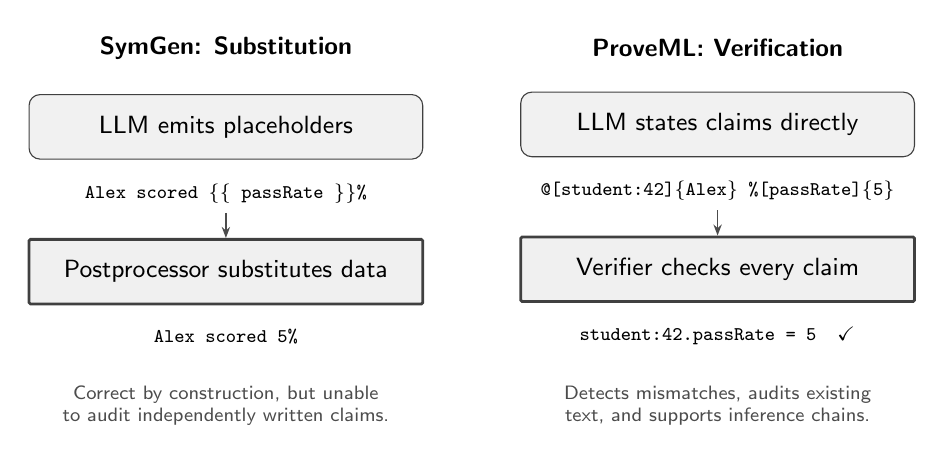
\begin{tikzpicture}[
    node distance=0.45cm and 0.6cm,
]
% SymGen side
\node[diag title] (st) {SymGen: Substitution};
\node[diag ai, below=0.32cm of st, minimum width=5.0cm] (sg1) {LLM emits placeholders};
\node[diag code, below=0.18cm of sg1] (sg1c) {\texttt{Alex scored \{\{ passRate \}\}\%}};
\node[diag det, below=0.32cm of sg1c, minimum width=5.0cm] (sg2) {Postprocessor substitutes data};
\node[diag code, below=0.18cm of sg2] (sg2c) {\texttt{Alex scored 5\%}};
\draw[diag arrow] (sg1c) -- (sg2);

\node[diag note, below=0.28cm of sg2c, text width=4.7cm] (sgnote) {Correct by construction, but unable to audit independently written claims.};

% ProveML side
\node[diag title, right=2.8cm of st] (pt) {ProveML: Verification};
\node[diag ai, below=0.32cm of pt, minimum width=5.0cm] (pm1) {LLM states claims directly};
\node[diag code, below=0.18cm of pm1] (pm1c) {\texttt{@[student:42]\{Alex\} \%[passRate]\{5\}}};
\node[diag det, below=0.32cm of pm1c, minimum width=5.0cm] (pm2) {Verifier checks every claim};
\node[diag code, below=0.18cm of pm2] (pm2c) {\texttt{student:42.passRate = 5 ~\checkmark}};
\draw[diag arrow] (pm1c) -- (pm2);

\node[diag note, below=0.28cm of pm2c, text width=4.7cm] (pmnote) {Detects mismatches, audits existing text, and supports inference chains.};
\end{tikzpicture}
\caption{Architectural comparison. SymGen prevents errors by substituting placeholders with data values. ProveML detects errors by verifying independently claimed values against the fact store.}
\label{fig:symgen-vs-proveml}
\end{figure}

\section{Reference Implementation}
\label{sec:implementation}

A reference implementation is available as a markdown-it plugin (JavaScript):

\begin{itemize}
    \item ProveML plugin (parser + renderer with lexical scope stack): 550 lines of JavaScript
    \item Threshold registry: 21 example thresholds, exercising the full operator vocabulary of Table~\ref{tab:operators}
    \item Test suite: 220 tests (137 plugin, 34 grammar, 15 paper examples, 14 CLI, 20 detection)
    \item Convergence harness: 28 prompts, 4 models, 3 repeats (Section~\ref{sec:education})
\end{itemize}

\paragraph{Fact store construction.} The experiment harness loads a JSON data file and flattens it into a key-value store at startup: each entity's fields become \texttt{type:id.field $\rightarrow$ value} entries. Optional \texttt{.\_unit} companion keys are added where units are declared. The flattening is a single pass over the source data with no external dependencies.

\paragraph{Verify-fix loop.} The generation pipeline calls the LLM, passes the response to the standalone verifier, and inspects the result. If errors remain and the loop budget is not exhausted, a correction prompt is constructed containing the specific verification errors and the original data context. The corrected response is accepted only if it improves verification without dropping claims.

\paragraph{Rendering integration.} The markdown-it plugin implements the same verification semantics against the same fact store and threshold registry as the standalone verifier (which is the normative component), then emits HTML spans with \texttt{data-*} attributes carrying the verification status, entity path, and error details. A CSS layer maps these attributes to visual indicators. The plugin and standalone verifier share the same fact store and threshold registry but are independently usable. That sameness is a maintained invariant rather than a given: an audit during the preparation of this paper found the plugin had drifted to two-valued condition evaluation, which rendered the negation of an unregistered threshold as verified; the suite now pins the two implementations to each other on exactly these cases.

\paragraph{Trust adapters.} The implementation also carries a layer this specification deliberately does not cover: a fact store can be wrapped in a \textit{trust adapter} that attaches a trust status (\texttt{verified}, \texttt{unverified}, \texttt{expired}, \texttt{revoked}, \texttt{error}) and a proof reference to each resolved value --- for stores backed by signed sources such as verifiable credentials --- and verification results merge these worst-first, so one revoked input marks every claim it touched. Claim verification and source trust stay orthogonal: a claim can match a value whose signature has expired, and the result carries both facts separately. The adapter interface ships with the package; its semantics are implementation-documented rather than specified here, and nothing in Sections \ref{sec:syntax}--\ref{sec:guarantee} depends on it.

\noindent Tested using a generated dataset in the shape of a secondary school assessment platform. Every record is drawn from the model described in Section~\ref{sec:evaluation}, none is derived from a real pupil, and the school does not exist. The reference implementation is available as an npm package (\texttt{proveml}) with source at \url{https://github.com/abovebeyond-ai/proveml}. The paper, benchmarks, experiment results, and reproducibility guide are at \url{https://github.com/abovebeyond-ai/proveml-research}.

\section{Discussion}

\subsection{What the Boundary Is For}

Although ProveML can improve output quality through verify-fix loops, its more durable contribution is the boundary it draws: a line inside a document separating claims that carry a machine-checkable status and a path back to a record from text that carries neither.

The verify-fix loop is a consequence of this design. Because verification is deterministic and instant, errors can be fed back to the LLM with specific messages (``\texttt{\%[passRate]\{7\} in student:42: should be 5}''), enabling targeted correction at claim-level granularity. But the loop is most useful for models that already produce well-formed markup. Without adequate context scaffolding, models may produce too little verifiable markup for the loop to help. For the most capable models, verification serves primarily as an audit trail. The loop's value is in the transition zone where models are capable enough to produce markup but not reliable enough to get it right on the first pass.

The deeper value is not the loop but the boundary itself. With ProveML markup, every marked claim carries a verification status and an addressable path, so a reader --- or an auditor months later --- can ask of any given number where it came from and get an answer that does not depend on a model. Prose without that structure can still be checked, but only in the aggregate and only by someone willing to re-derive it. What changes is the unit of accountability: from ``was this report right'' to ``was this claim right, and against which record''.

\subsection{Incentive-Aligned Generation}

A key design goal of ProveML is that the markup language should be \textit{easy for LLMs to use correctly}. This is not incidental; it creates a productive alignment between the model's generation objective and the system's verification objective.

\paragraph{Maximizing verifiable surface area.} A deployment's system prompt sets how much of the output it asks to be marked: at minimum every entity in \texttt{@[entity:id]\{name\}} and every number in \texttt{\%[field]\{value\}}, and where qualitative language matters, every judgment in \texttt{?[label: THRESHOLD]\{text\}}. The more a prompt asks for, the more of the response arrives as verifiable constructs and the smaller the residue of unchecked prose, which is what the coverage audit in Section~\ref{sec:coverage} measures. The prompt used throughout our evaluation asks only for the first two, so the numbers reported here describe entity and fact markup and say nothing about how well models produce inference constructs; that is a gap in the evaluation, not a property of the language, and Section~\ref{sec:limitations} states it as such.

\paragraph{Why LLMs are well-suited to this.} Three properties of modern LLMs make ProveML generation natural rather than burdensome:

\begin{enumerate}
    \item \textbf{Markdown fluency}: LLMs are extensively trained on Markdown and produce it natively. ProveML's constructs (\texttt{@[...]}, \texttt{\%[...]}, \texttt{?[...]}) use characters that do not conflict with Markdown syntax, making them easy to interleave with natural language.
    \item \textbf{In-context learning}: A few examples in the system prompt are sufficient for LLMs to adopt the ProveML pattern in practice. Prompt examples alone were enough for every model we tested to adopt the pattern, with no fine-tuning (Section~\ref{sec:education}).
    \item \textbf{Structured data access}: When the fact store is provided in the context window, the model has direct access to the exact values it should reference. The task reduces to \textit{selecting and formatting} rather than \textit{recalling from parametric memory}, precisely the setting where LLMs are most reliable.
\end{enumerate}

\paragraph{Model-agnostic by design.} ProveML deliberately avoids requiring fine-tuned or specialized models. The system prompt, fact store, threshold registry, and verify-fix loop together form a \textit{skill} that any general-purpose LLM can execute. As foundation models improve, ProveML benefits automatically: fewer first-pass errors, fewer correction iterations. The right abstraction is not ``train the model to be more verifiable'' but ``give the agent the tools to prove its claims.''

\subsection{The Claim Boundary: Domain Experts Define What Can Be Stated}
\label{sec:boundary}

Not every sentence in AI-generated text needs to be a verified claim. The goal is not to annotate 100\% of the prose, but to give domain experts a precise way to mark which claims should be checked. This creates a clear boundary between two modes of AI output:

\begin{enumerate}
    \item \textbf{Verified claims}: facts, entity references, and inferences that resolve against the fact store and threshold registry. These are rendered with verification indicators and can be trusted to be consistent with the data.
    \item \textbf{Plain prose}: text outside ProveML markup. It remains ordinary prose with no verification status and should not be treated as a checked claim.
\end{enumerate}

The threshold registry defines which qualitative judgments \textit{can} be verified. Claims inside the registry get checked deterministically. Text outside the markup remains unchecked prose. Deployments may prompt for broader use of markup, but ProveML itself does not scan or reject plain prose outside the verified layer.

In practice, the system prompt can encourage authors to keep consequential judgments inside the verified layer:

\begin{lstlisting}
RULES:
- Every qualitative word MUST use ?[label: THRESHOLD]{text}
- If no threshold exists for your observation, write it as:
  "This may warrant further investigation" (NOT "This is X")
\end{lstlisting}

\noindent If the AI writes an unregistered threshold name inside a ProveML construct, the verifier returns an error. Otherwise, plain prose remains unchecked.

\paragraph{Progressive adoption.} Adoption is not all-or-nothing. At Level 1 (entity references and fact values only), ProveML already detects wrong numbers. At Level 2, the threshold registry constrains qualitative language. Deploying requires only addressable data and, optionally, threshold definitions --- a flat configuration file per domain. The verifier, grammar, and verify-fix loop are unchanged across domains. The design also extends naturally to settings with machine-verifiable attestations (verifiable credentials, SSI systems, blockchain-derived state), though these applications are forward-looking and not evaluated in this paper.

\subsection{Scope and Privacy}

ProveML verifies what the AI \textit{marks up}: every entity name, every number, and every thresholded qualitative judgment inside a ProveML construct. Text outside the markup remains unchecked prose. The system's guarantee is ``consistent with the fact store.'' The fact store is the single point of trust.

\paragraph{Privacy by design.} Because entity references are structural (\texttt{@[student:42]\{...\}}) and the display text is separate from the identifier the verifier resolves, a deployment can hand the model pseudonymous identifiers and have the rendering layer substitute names at display time: the verification status travels with the markup, the identifying data stays behind. This is a property the syntax makes available, not one it enforces, and our evaluation does not use it --- the benchmark contexts carry generated pupil names and the models write them out. Whether a pseudonymous configuration costs anything in markup quality is untested.

\subsection{Limitations}
\label{sec:limitations}

\begin{itemize}[nosep]
    \item \textbf{Consistency, not truth.} ProveML verifies that claims match the fact store, not that the fact store is correct. If the source data is wrong, verified claims will be wrong. The review layer described under Deployment gives that boundary a discipline --- evidence per store value, a human sign-off saved under a hash of exactly what it judged, expiring when the evidence changes --- but does not remove it: a fair reading is a judgement, not a proof.
    \item \textbf{The right name, not necessarily the right record.} An entity verifies when the name the reader sees equals the name stored at the id the model chose; nothing checks that the model chose the right id. If two records of one type share a name, a wrong id renders identically to the right one and only the audit path tells them apart. The verifier therefore measures whether a rendered subject is unique in the store (\texttt{subjectUnique}: true, false with the other paths, or unknown when the source cannot be enumerated), \texttt{doctor} warns on duplicate names, strict mode makes an ambiguous subject a finding, and the render marks it. Where subjects are identifiers by construction, as on a ledger, the gap closes; where they are personal names, it does not, and the marker is what remains.
    \item \textbf{No unit conversion.} Units are supported as nullable metadata with exact string matching. Semantic unit equivalence (e.g., mg/dL vs mmol/L) and standardized vocabularies (UCUM~\citep{ucum}, ISO 4217~\citep{iso4217}) are deferred to future work.
    \item \textbf{Evaluation scope.} The evaluation covers two domains (generated education, real SEC finance) across 38 prompts, 4 models, and 3 repeats. Whether error patterns generalize to larger schemas, more domains, or frontier models is not exhaustively established.
    \item \textbf{Judgments: one domain, one registry.} The judgment study of September 2026 (reported in the short paper) covers one store, one registry of fourteen names and twenty questions; the local-model runs in this report predate it and asked for entities and facts only. How the construct behaves with a large registry, with judgments over derived values, or when the registry itself is contested, is not measured.
    \item \textbf{Canonical claims.} The model is not allowed to round: a claim says \texttt{391035000000}, never ``\$391 billion''. The reader can still see the rounded form, because the store may declare a display rule per field (\texttt{\_display}) that the renderer applies to verified values; but a value the model itself rounded is a mismatch, and prose that quotes the rounded figure outside a claim is unverified prose. The rule is on the store's side of the boundary on purpose: a tolerance in the verifier would make ``about 18'' verify against 18.5 and turn the guarantee into an approximation.
    \item \textbf{Prose outside markup.} ProveML verifies what is inside markup constructs. Text outside the markup is not checked; detecting unverified claim-bearing prose is outside the scope of the current specification. Section~\ref{sec:coverage} quantifies the numeric portion of this gap: coverage ranges from 60.5\% to 91.9\% depending on model, benchmark, and prompt language.
    \item \textbf{Malformed input.} The tokenizer silently skips constructs with unmatched brackets or braces. Robustness to diverse malformed markup deserves further stress-testing.
    \item \textbf{Adversarial generation.} ProveML is designed against models that make mistakes, not against a model trying to mislead. A generator that wanted to could choose a threshold that holds and wrap misleading words around it, mark only the claims that verify and leave the damaging ones as prose, or select a true fact that misrepresents the record it came from. Each of these survives verification because the verifier reads paths and values, not intent. We neither measure nor defend against this.
    \item \textbf{Group claims.} Inferences evaluate against a single entity context. A claim like ``5TW, 4B, and 6WE all have low coverage'' cannot be verified as one inference; it must be decomposed into one inference per entity.
\end{itemize}

\subsection{Future Work}

Several extensions are deferred from the current specification: (1) standardized unit vocabularies (UCUM~\citep{ucum}, ISO 4217~\citep{iso4217}) for semantic unit equivalence rather than string matching; (2) multiple fact stores with explicit source provenance or a source prefix on entity paths; (3) cross-implementation portability of canonicalization rules; (4) derived-value claims (counts, differences, ratios computed from store values), which the current specification cannot express as facts at all (Section~\ref{sec:coverage}); (5) tolerance-based matching and display-time formatting for rounded prose; (6) further ablations separating context size from domain and prompt mix (prompt language is ablated in Section~\ref{sec:langablation}); and (7) evaluation on larger schemas, more domains, and frontier models, with an abstention metric for unsupported queries.

\section{Conclusion}

ProveML places AI-generated claims inside a verifiable boundary. Three inline constructs link every claim to an addressable path in a data source. Verification is deterministic, with no model in the loop. An optional threshold registry extends this to qualitative judgments through composable primitives.

In our evaluation across four models (3.8B to API-scale, 3 runs each), we find that the capability threshold depends strongly on the shape of the request rather than on model size: on an educational benchmark with 95 class offerings and 741 students, Phi-3 scored 38\% $\pm$ 33.7 with individual runs at 65\%, 48\% and 0\%; on a compact SEC EDGAR finance benchmark (2 entities), the same model scored 92\% $\pm$ 2.5 with all three runs within 5 points, the architecture, verifier, and grammar unchanged. Ablations locate two of the responsible factors: within the educational benchmark, prompt language moves this smallest model roughly 22 percentage points and the larger three almost nothing, and giving any local model the full dataset instead of a slice drives markup production to zero --- not to silence, but to unverifiable prose.

What LLMs provide is open-ended generation. What ProveML adds is a controllable, auditable boundary around that generation. For humans, the intended benefit is visual triage: verified claims carry a status, and attention shifts to what is unverified. We have not measured whether this reduces human verification effort, and the evidence from adjacent systems is mixed: \citet{symgen} report their user study reduced average verification time by 20\%, while \citet{ten2026} report a 21-participant study in which verification and correction effort did not differ significantly from their baseline, even though their system reduced hallucination. Which of the two ProveML's rendering resembles in practice is an open empirical question. For agent loops the benefit is more direct and does not depend on human factors: specific error feedback (``\texttt{\%[glucose]\{143 mg/dL\} in patient:308: should be 142 mg/dL}'') enables targeted self-correction, which is what the verify-fix loop measures in Section~\ref{sec:evaluation}. The combination is what neither open-ended generation nor static verification offers alone: open-endedness with determinism.

\section*{Declaration of Generative AI Use}

Generative AI tools (Claude, GPT) were used during manuscript preparation for drafting, revision, literature search, and code review. All AI-generated content was reviewed, verified, and edited by the author. No generative AI was used to create or alter images or artwork. The author takes full responsibility for the content of the published article.

\bibliographystyle{plainnat}
\bibliography{proveml}

\appendix

\section{Error Detection Rate}
\label{sec:detection}

\paragraph{Setup.} The critical question for ProveML is not whether the LLM generates correct output, but whether ProveML \textit{detects} incorrect output. To test this, we injected 20 deliberate errors into otherwise valid ProveML text and measured whether the verifier caught each one.

\paragraph{Results.} The 20 errors span six categories: wrong values (5), wrong entity (3), no context (2), wrong threshold (4), cross-entity swaps (2), and subtle errors including trailing spaces and swapped entity order (4). ProveML detected all 20, yielding a \textbf{100\% error detection rate}. This is a consequence of deterministic equality checking: if the claimed value does not exactly match the fact store, the claim is flagged regardless of plausibility. The experiment validates that the implementation behaves as specified --- it is a conformance test, not a detector benchmark --- and it is one-sided: it measures detection of planted errors, not false positives on correct-but-reformatted values (a canonicalization difference such as \texttt{18.50} vs.\ \texttt{18.5} is flagged despite numeric equality; see Section~\ref{sec:limitations}). Robustness to malformed LLM markup is partially addressed by the convergence experiment (Section~\ref{sec:education}) but deserves further stress-testing.

\section{ProveML Grammar (EBNF)}
\label{app:grammar}

The following EBNF captures the ProveML constructs as implemented in the reference parser. It is intended as a starting point for formal treatment, not a normative specification; the authoritative definition is the reference implementation and test suite. Where the two diverge, the reference tokenizer is deliberately \textit{more permissive} than this grammar --- for example, it accepts identifiers beyond the character classes below and tolerates a missing space after the inference label colon --- so the grammar describes the canonical surface form generators should produce, while the tokenizer accepts sloppier variants of it. One exception runs the other way: the tokenizer brace-counts entity display text, so an unbalanced open brace (admitted by the \texttt{display\_text} production) causes the construct to be skipped.

\begin{lstlisting}
(* ProveML constructs inside Markdown inline content *)
entity_ref_simple = "@[" , entity_path , "]{" , display_text , "}" ;
entity_ref_scoped = "@[" , entity_path , " " , DQUOTE ,
                    entity_name , DQUOTE , "]{" ,
                    scoped_content , "}" ;
entity_ref        = entity_ref_simple | entity_ref_scoped ;

fact_ref          = "%[" , field_name , "]{" , value_text , "}" ;
inference_ref     = "?[" , label , ": " , condition , "]{" ,
                    display_text , "}" ;

(* Paths and identifiers *)
entity_path       = identifier , ":" , entity_id ;
entity_id         = ( letter | digit ) ,
                    { letter | digit | "_" | "-" } ;

field_name        = field_segment , { "." , field_segment } ;
field_segment     = meta_field | path_field | identifier ;
meta_field        = "_" , identifier ;
path_field        = identifier , ":" , entity_id ;

label             = identifier ;
identifier        = letter , { letter | digit | "_" } ;

(* Text content *)
entity_name       = { char - '"' - ']' } ;
display_text      = { char - "}" } ;
scoped_content    = { char } ;   (* parsed recursively *)
value_text        = { char - "}" } ;

(* Condition grammar *)
condition         = or_expr ;
or_expr           = and_expr , { " OR " , and_expr } ;
and_expr          = unary_expr , { " AND " , unary_expr } ;
unary_expr        = [ "NOT " ] , primary ;
primary           = threshold_name
                  | threshold_name , "(" , path , ")"
                  | "@" , label ;

(* Terminals *)
threshold_name    = uppercase , { uppercase | digit | "_" } ;
path              = entity_path , "." , field_name ;
DQUOTE            = '"' ;
letter            = "a"-"z" | "A"-"Z" ;
uppercase         = "A"-"Z" ;
digit             = "0"-"9" ;
\end{lstlisting}

\end{document}
